\documentclass[journal,twoside,web]{ieeecolor}
\usepackage{generic}
% \usepackage[outdir=./figs]{epstopdf}
% \usepackage{epstopdf}
%\usepackage{cite}
\let\proof\relax
\let\endproof\relax
\let\labelindent\relax
\usepackage{amsmath,amssymb,amsfonts,amsthm}
\usepackage[font=small]{caption}
\usepackage[font=small]{subcaption}
\usepackage{algorithmic}
\usepackage{graphicx}
\usepackage{textcomp}
\usepackage[ruled]{algorithm2e}
\SetKw{Break}{break}
\SetKw{Continue}{continue}
\setlength{\marginparwidth}{2cm}
% \usepackage{todonotes}
%\usepackage{sample_complexity_hanchmin/hanch_sty}
\usepackage{cuted}
\usepackage{enumitem}
\setitemize{noitemsep,topsep=0pt,parsep=0pt,partopsep=0pt}
\usepackage{dsfont}
%\usepackage{xstring}
\usepackage{orcidlink}
\usepackage[backend=biber,style=numeric-comp,sorting=none,natbib=true,doi=false,isbn=false,url=false,eprint=false,giveninits=true]{biblatex}
\addbibresource{references.bib}
\usepackage{tikz}
\usetikzlibrary{automata, positioning}
\usepackage{pgfplots}
\usepackage{pgfplotstable} % For reading CSV files

\usepgfplotslibrary{fillbetween} 
\pgfplotsset{compat=1.17}
\usepgfplotslibrary{colormaps}
%\definecolor{mycolorZ0}{RGB}{100,50,50}%brown
%\definecolor{mycolorZ2}{RGB}{255,0,0}%red
%\definecolor{mycolorZ4}{RGB}{255,200,200}%pink
%\definecolor{mycolorZ5}{RGB}{200,80,200}%magenta
%\definecolor{mycolorZ1}{RGB}{255,150,0}%orange
%\definecolor{mycolorZ3}{RGB}{100,30,255}%purple

\definecolor{mycolorZ0}{named}{red}%red
\definecolor{mycolorZ1}{named}{green}%green
\definecolor{mycolorZ2}{named}{blue}%blue
\definecolor{mycolorZ3}{named}{orange}%orange
\definecolor{mycolorZ4}{named}{cyan}%cyan
\definecolor{mycolorZ5}{named}{magenta}%magenta


\definecolor{mycolorA0}{RGB}{0,0,255}%blue
\definecolor{mycolorA3}{RGB}{0,200,0}%light green
\definecolor{mycolorA2}{RGB}{0,100,0}%dark green
\definecolor{mycolorA1}{RGB}{0,200,200}%cyan
\definecolor{mycolorA4}{RGB}{50,50,50}%grey

%\usepackage{natbib}
% \usepackage{academicons}
% \newcommand{\orcidlogo}{\href{https://orcid.org/0009-0000-4783-0632}{\textsuperscript{\includegraphics[scale=0.08]{TAC_journal/logo-orcid-eps-converted-to.pdf}}}}
%\usetikzlibrary{external}
%\tikzexternalize[prefix=./]
% \theoremstyle{definition}
\newtheorem{definition}{Definition}
\newtheorem{remark}{Remark}
\newtheorem{lemma}{Lemma}
\newtheorem{claim}{Claim}
\newtheorem{theorem}{Theorem}
\newtheorem{corollary}{Corollary}
\newtheorem{proposition}{Proposition}
\newtheorem{assumption}{Assumption}
\newtheorem{innercustomthm}{Theorem}
\newenvironment{customthm}[1]
  {\renewcommand\theinnercustomthm{#1}\innercustomthm}
  {\endinnercustomthm}
 \newtheorem{innercustomlem}{Lemma}
\newenvironment{customlem}[1]
  {\renewcommand\theinnercustomlem{#1}\innercustomlem}
  {\endinnercustomlem}
  
% \renewcommand{\baselinestretch}{.985}
\renewcommand{\baselinestretch}{1}

\DeclareMathOperator*{\argmax}{argmax} \allowdisplaybreaks
  
\usepackage{ifthen}
\newboolean{showcomments}
\setboolean{showcomments}{true}
% \usepackage[usenames,dvipsnames]{xcolor}
% \usepackage[usenames,dvipsnames]{color}
\usepackage{todonotes}

% \newboolean{resubmission}
% \setboolean{resubmission}{true}
% \newcommand{\resubmit}[1]{
% \ifthenelse{\boolean{resubmission}}{
% \textcolor{blue}{#1}
% }
% {}
% }
% \newcommand{\resubmit}[1]{\textcolor{blue}{#1}}

\newtheorem{example}{Example}

\newboolean{arxiv}
\setboolean{arxiv}{false}

\definecolor{bleudefrance}{rgb}{0.19, 0.55, 0.91}
\definecolor{ao(english)}{rgb}{0.0, 0.5, 0.0}

%ADD CITES
\newcommand{\addcite}[0]{\ifthenelse{\boolean{showcomments}}
{\textcolor{purple}{(add cite(s)) }}{}}%

\newcommand{\addcites}[0]{\ifthenelse{\boolean{showcomments}}
{\textcolor{purple}{(add cite(s)) }}{}}%

% Comments
\newcommand{\leopoldo}[1]{  \ifthenelse{\boolean{showcomments}}
{\todo[inline,color=bleudefrance]{Leopoldo: #1}}{}}

\newcommand{\juan}[1]{  \ifthenelse{\boolean{showcomments}}
{\todo[inline,color=pink]{Juan: #1}}{}}

\newcommand{\santiago}[1]{  \ifthenelse{\boolean{showcomments}}
{\todo[inline,color=orange]{Santiago: #1}}{}}

\newcommand{\miguel}[1]{  \ifthenelse{\boolean{showcomments}}
{\todo[inline,color=purple!60!white]{Miguel: #1}}{}}

\newcommand{\sean}[1]{  \ifthenelse{\boolean{showcomments}}
{\todo[inline,color=green!60!white]{Sean: #1}}{}}


%Edits to be highlighted
\newboolean{showedits}
\setboolean{showedits}{true}
\usepackage[markup=underlined]{changes}
\definechangesauthor[color=bleudefrance]{EM}
\newcommand{\aem}[1]{
\ifthenelse{\boolean{showedits}}
{\added[id=EM]{#1}}
{\!#1\hspace{-4.75pt}}
}
\newcommand{\repem}[2]{
\ifthenelse{\boolean{showedits}}
{\replaced[id=EM]{#1}{#2}}
{\!#1\hspace{-4.75pt}}
}
\newcommand{\dem}[1]{
\ifthenelse{\boolean{showedits}}
{\deleted[id=EM]{#1}}
{}
}

\newcommand{\hl}[1]{#1}
% \renewcommand{\hl}[1]{\textcolor{black}{#1}}
%\listoftodos[{\color{red}\textbf{List of comments/suggestions}}]

  
\def\BibTeX{{\rm B\kern-.05em{\sc i\kern-.025em b}\kern-.08em
    T\kern-.1667em\lower.7ex\hbox{E}\kern-.125emX}}
\markboth{\journalname, VOL. XX, NO. XX, XXXX}
{Leopoldo Agorio \MakeLowercase{\textit{et al.}}: 
Cooperative Multi-Agent Assignment over Stochastic Graphs via Constrained Reinforcement Learning
}

\begin{document}
\title{
Cooperative Multi-Agent Assignment over Stochastic Graphs via Constrained Reinforcement Learning
}

%\author{Leopoldo Carlos Agorio Grove\orcidlink{XXXX-XXXX-XXXX-XXXX}, \IEEEmembership{Student Member, IEEE}, Santiago Paternain\orcidlink{XXXX-XXXX-XXXX-XXXX}, \IEEEmembership{Member, IEEE},\\
 %Miguel Calvo-Fullana\orcidlink{XXXX-XXXX-XXXX-XXXX},\IEEEmembership{Member, IEEE} , and Juan Andres Bazerque\orcidlink{0000-0001-9950-1208},
 %\IEEEmembership{Member, IEEE}
%\thanks{}\thanks{}\thanks{}\thanks{}\thanks{}
%
%\author{Leopoldo Agorio\href{https://orcid.org/0009-0000-4783-0632}{\includegraphics[scale=0.08]{logo-orcid-eps-converted-to.pdf}}, \IEEEmembership{Student Member, IEEE}, Sean Van Alen\href{https://orcid.org/0009-0000-4783-0632}{\includegraphics[scale=0.08]{logo-orcid-eps-converted-to.pdf}}, \IEEEmembership{Student Member, IEEE}, 
 %       Santiago Paternain\href{https://orcid.org/0009-0000-4783-0632}{\includegraphics[scale=0.08]{logo-orcid-eps-converted-to.pdf}}, \IEEEmembership{Member, IEEE},
  %      Miguel Calvo-Fullana\href{https://orcid.org/0009-0000-4783-0632}{\includegraphics[scale=0.08]{logo-orcid-eps-converted-to.pdf}}, \IEEEmembership{Member, IEEE}, and 
   %     Juan Andres Bazerque\href{https://orcid.org/0009-0000-4783-0632}{\includegraphics[scale=0.08]{logo-orcid-eps-converted-to.pdf}}, \IEEEmembership{Member, IEEE}
%}


\author{Leopoldo Agorio, Sean Van Alen, 
         Santiago Paternain,
        Miguel Calvo-Fullana, and 
        Juan Andres Bazerque      
        % <-this % stops a space
\thanks{Leopoldo Agorio, Sean Van Allen, and Juan Andres Bazerque are with the Dept. of Electrical and Computer Engineering, Univ. of Pittsburgh, Pittsburgh, PA, USA  (emails: lca31@pitt.edu, sgv13@pitt.edu, juanbazerque@pitt.edu). \\
%
Santiago Paternain is with the 
Dept. of Electrical Computer and Systems Engineering, Rensselaer Polytechnic Institute, Troy, NY, USA (e-mail: paters@rpi.edu).\\
%
Miguel Calvo-Fullana is with the Dept of Engineering,  Universitat Pompeu Fabra, Barcelona, Spain (email: miguel.calvo@upf.edu). }}
\maketitle

\begin{abstract}
  Constrained multi-agent reinforcement learning offers the framework to design scalable and almost surely feasible solutions for teams of agents operating in dynamic environments to carry out conflicting tasks. We address the challenges of multi-agent coordination through an unconventional formulation in which the dual variables are not driven to convergence but are free to cycle, enabling agents to adapt their policies dynamically based on real-time constraint satisfaction levels. The coordination relies on a light single-bit communication protocol over a network with stochastic connectivity. Using this gossiped information, agents update local estimates of the dual variables. Furthermore, we modify the local dual dynamics by introducing a contraction factor, which lets us use finite communication buffers and keep the estimation error bounded. Under this model, we provide theoretical guarantees of almost sure feasibility and corroborate them with numerical experiments in which a team of robots successfully patrols multiple regions, communicating under a time-varying ad-hoc network. 
\end{abstract}

\section{Introduction}
\section{Introduction}
\label{sec:intro}


\ps{Challenges of technology scaling}

The growing demand for computing performance has always been met by increasing the number of transistors per chip, which is only possible due to CMOS technology scaling.
However, as we keep pushing the boundaries of technology scaling, we encounter multiple challenges.
Firstly, whenever we transition to a more advanced technology node, the non-recurring cost due to physical design, verification, software, mask sets, and prototyping almost doubles \cite{cost-tech-node}.
As a result, designing a chip in an advanced technology node is only economically viable if the chip is manufactured in vast quantities.
Secondly, many chip components such as I/O drivers, analog circuits, or \gls{srams} have reached their scaling limit.
This means that we cannot shrink these components further, even if we use a more advanced technology with a smaller feature size.
Thirdly, advanced technology nodes suffer from high defect rates, diminishing the yield and inflating the recurring cost.
To tackle these challenges, new chip-design paradigms have been developed.

\ps{Why 2.5D integration?}

One of these new paradigms is 2.5D integration, where multiple silicon dies called chiplets are integrated into the same package.
Once designed, a single chiplet can be reused in multiple 2.5D stacked chips, which increases the ratio of production volume to non-recurring cost.
Another advantage is that multiple chiplets - fabricated in different technologies - can be integrated into the same package.
This means that only components that can take full advantage of technology scaling are built in bleeding-edge technologies.
Components that have reached their scaling limit are fabricated in more mature and hence less costly technology nodes.
Furthermore, chiplets are smaller than monolithic chips.
Therefore, manufacturing chiplets results in less silicon area loss due to fabrication defects and hence a higher yield.
Due to these economic advantages, chip vendors such as AMD \cite{amd-chiplet} and NVIDIA \cite{chiplet-book} have adopted the 2.5D integration paradigm.  

\ps{Challenges of 2.5D integration}

An important challenge when designing 2.5D stacked chips is the construction of a low-latency and high-throughput \gls{ici}. 
To build an \gls{ici}, we connect different chiplets using \gls{d2d} links.
These links are fabricated in an organic package substrate, silicon bridge, or silicon interposer, and they are connected to the chiplets using \gls{c4} bumps or microbumps.
The number of bumps per chiplet is limited, and so is the bandwidth of \gls{d2d} links.
In addition to having lower bandwidth than links in monolithic chips, \gls{d2d} links also have higher latency.
This latency is caused by wire delay and by \gls{phys} that are necessary in both the sending and the receiving chiplet.
\gls{phys} are needed to convert between protocols, voltage levels, and frequencies, which are usually different between on-chiplet links and \gls{d2d} links.
Due to these limitations, the \gls{ici} can quickly become a bottleneck.

\ps{How we solve these challenges differently than the related work does.}

Existing approaches to maximize the performance of the \gls{ici} either optimize the placement of chiplets (with potentially heterogeneous shapes) for a predetermined \gls{ici} topology 
\cite{ho,liu,seemuth,eris,osmolovskyi,tap25d,chiou}, select one topology out of a set of candidates \cite{coskun-1, coskun-2}, or they optimize the \gls{ici} topology for a 2D grid of homogeneously shaped chiplets on an active interposer \cite{butterdonut, cluscross, kite}.
To the best of our knowledge, there is no prior work on \gls{ici} topologies for chips with heterogeneously shaped chiplets or with passive silicon interposers or silicon bridges.
To fill this gap, we propose \name, a novel optimization methodology to jointly optimize the chiplet placement and \gls{ici} topology of such architectures.
\ifnb
\else
\newpage
\fi

\ps{Details on \name~and the key idea}

The key idea is as follows: 
We optimize the chiplet placement without a predetermined topology.
For each placement generated by an optimization algorithm, we infer a placement-based \gls{ici} topology by connecting chiplets that are in close proximity in that specific placement.
We then compute the latency and throughput of this combination of placement and topology for different traffic types.
These latencies and throughputs together with the total chip area are used to compute a user-defined quality-score of the placement, which is returned to the optimization algorithm.
Based on this quality score, the algorithm can further optimize the placement.
By following this iterative process, we jointly optimize the chiplet placement and the \gls{ici} topology.

\ps{Short evaluation-summary}

We provide our open-source framework implementing the proposed placement and topology co-optimization methodology, which we evaluate using both synthetic traffic and traffic traces.
A 2D grid of chiplets with a mesh topology is used as a baseline since many proposals for 2.5D stacked chips \cite{dataflow_accel_dnn, cifher, simba, hecaton, dojo} use such an architecture.
We reduce the latency of synthetic L1-to-L2 and L2-to-memory traffic, the two most important traffic types for cache coherency traffic, by up to 28\% and 62\% respectively.
For real traffic traces, we reduce the average packet latency for almost all traces and architectures considered (reduced by an 8\% or 18\% on average depending on the configuration of \gls{phys} within a chiplet).


\section{Problem Formulation}
\label{sec:problem_form}

Consider $N$ agents interacting with an environment that is modeled as an MDP with transition probabilities $\mathbb{P}\left(S_{t+1}\mid S_{t},A_{t}\right)$. For each time index $t=0,1,2,\ldots$, random variables $S_t=(S_t^1,\ldots,S_t^N)$ and $A_t=(A_t^1,\ldots,A_t^N)$ collect the states $S_t^n\in \mathcal S$ and actions $A_t^n\in \mathcal A$ for all agents. The team receives a vector of rewards $r(S_t)\in \mathbb R^M$ associated with $M$ different tasks that must be collectively satisfied. We consider a family of assignment problems in which the agents must persistently cover $M$ regions of the state space denoted by $\mathcal{S}_m\subset\mathcal{S}$ with $m=1,\ldots,M$. Thus, each reward is given by
%
\begin{equation}\label{eqn_patrolling_reward}
%    r_m(S_t,A_t) = \max_{n=1,\ldots,N} \mathds{1}[S_{tn}\in \mathcal{S}_m]
    \left(r(S_t)\right)_m = \max_{n=1,\ldots,N} \mathds{1}[S_t^n\in \mathcal{S}_m],
\end{equation}
where  $\left(r\right)_m$ represents the $m$-th element of vector $r$,  with the index function defined as
    $\mathds{1}[S_t^n\in \mathcal{S}_m]=1 $ if $  S_t^n\in \mathcal{S}_m$ and zero otherwise. %,
%
Each region $\mathcal S_m$ must be covered by the agents a fraction of the time. Hence, we set the requirements as a vector $c\in[0,1]^M$ of $M$ thresholds on the average rewards, and formulate a Markov decision problem with constraints
\begin{equation}\label{eqn_ideal_V}
    V(\pi):= \lim_{T\to \infty}\frac{1}{T} \mathbb E_{S_t, A_t\sim \pi} \left [ \sum_{t=0}^{T-1} r(S_t) \right ] \geq c,
    \end{equation}
%
with the inequality being component-wise. The expectation is taken over the transition probabilities and the probability distribution defining the control policy $\pi(A_t|S_t)$  of the actions of all agents given their states.

A task reward can be incorporated to establish an optimization objective. This can be useful to set a secondary goal, such as minimizing energy consumption in a multi-robot application like the one presented in Example \ref{example} below. However, in the following, we will set the objective to zero and focus on our primary goal of satisfying the specifications.

Hence, the feasibility problem we aim to solve is
%
\begin{align}\label{eqn_crl}
P^\star = &\; \max_{{\pi}} 0\\*
\textrm{s. to} &\; \lim_{T\to \infty}\frac{1}{T} \mathbb E_{S_t, A_t\sim \pi} \left [ \sum_{t=0}^{T-1} r(S_t) \right ] \geq c.\notag 
\end{align}
%
To illustrate the practical use of this problem formulation, we include the following example, which we will explore further in the experiments of Section \ref{sec_numerical}.

\begin{example}\label{example}
Consider a team of $N$ robots that is required to monitor $M>N$ areas,  visiting areas $\mathcal S_1,\ldots,\mathcal S_M$ during fractions of time given by  $c\in [0,1]^M$. These conflicting requirements may not be achievable by a single robot, particularly when the aggregate thresholds are greater than one, i.e., $\left\|c\right\|_1>1$, and not even by multiple robots acting independently following the same optimal single-agent policy. Coordination is thus essential, for which robots can form an ad-hoc communication network. 
\end{example}
%



We aim to solve \eqref{eqn_crl} in a coordinated distributed fashion, in a scenario in which agents do not have access to the whole system state but can only observe their own state $S_t^n$. Once deployed, agents will not share their locations. Instead, we will develop a light gossip protocol for agents to exchange \emph{single-bit messages} with their neighbors (Section \ref{sec_online_execution}) over an ad-hoc communication network adhering to the stochastic graph model in \cite{Nedic2017Achieving}.  This graph model considers a time domain $\mathcal T \subset \mathbb N$ and a set of nodes $\mathcal V=\{1,\ldots,N\}$ representing the agents. Then, $\mathcal G = \mathcal G(\mathcal V,\mathcal E,\mathcal T, w_G)$ defines a stochastic graph where edges are sampled from a static underlying graph $G = (\mathcal V, \mathcal E)$. This \textit{footprint} graph $G$ indicates pairs of agents that could have connectivity at some point in time. In this model,  $G$ is assumed to be connected, but it is noteworthy that this does not necessarily imply that $\mathcal G$ is connected. Indeed, $\mathcal G$ could be disconnected at all times. Accordingly, the \textit{presence} function $w_G: \mathcal E \times \mathcal T \to \{0,1\}$ is included to indicate if an edge is present at a given time.
%
We will consider a probabilistic model in which the presence of an edge 
$e^{(n,n^\prime)} \in\mathcal{E}$ 
between two agents    $n,n^\prime \in \mathcal{V}$  at time $t$ is modeled as a Bernoulli random variable with probability $p$, i.e., 
%
\begin{align}
w_G\left(n,n^\prime,t\right)& \text{ are i.i.d. }  \text{Bernoulli}(p).\label{eqn_graph_model}
\end{align} 
Edges are independent of each other, as it is also the activation of an edge across time.   Figure \ref{fig:gossip_stochastic} illustrates the communication graph for the monitoring problem in Example \ref{example}.

\begin{figure}[t]
    \centering
    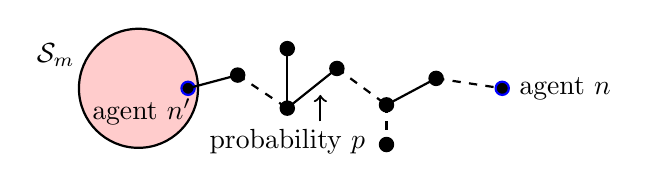
\begin{tikzpicture}[scale=0.42]

    % Main zones
    \filldraw[color=black, fill=red!20, thick] (0,0) circle (1.8cm); % Smaller zone around agent i
    \filldraw[color=blue, fill=black, thick] (1.5,0) circle (0.2); % Agent i
    \filldraw[color=blue, fill=black, thick] (11,0) circle (0.2); % Agent n

    % Intermediate nodes on a zigzag path between i and n
    \filldraw[color=black, fill=black, thick] (3,0.4) circle (0.2);    % Node 1 (slightly above)
    \filldraw[color=black, fill=black, thick] (4.5,-0.6) circle (0.2); % Node 2 (slightly below)
    \filldraw[color=black, fill=black, thick] (6,0.6) circle (0.2);    % Node 3 (slightly above)
    \filldraw[color=black, fill=black, thick] (7.5,-0.5) circle (0.2); % Node 4 (slightly below)
    \filldraw[color=black, fill=black, thick] (9,0.3) circle (0.2);    % Node 5 (slightly above)

    % Dotted line segments connecting nodes from agent i to agent n
    \draw[color=black, thick] (1.5,0) -- (3,0.4);
    \draw[color=black, thick,dashed] (3,0.4) -- (4.5,-0.6);
    \draw[color=black, thick] (4.5,-0.6) -- (6,0.6);
    \draw[color=black, thick, dashed] (6,0.6) -- (7.5,-0.5);
    \draw[color=black, thick] (7.5,-0.5) -- (9,0.3);
    \draw[color=black, thick,dashed] (9,0.3) -- (11,0);

    % Branching nodes
    \filldraw[color=black, fill=black, thick] (4.5,1.2) circle (0.2); % Branch above
    \draw[color=black, thick] (4.5,-0.6) -- (4.5,1.2);

    \filldraw[color=black, fill=black, thick] (7.5,-1.7) circle (0.2); % Branch below
    \draw[color=black, thick, dashed] (7.5,-0.5) -- (7.5,-1.7);

    % Arrow pointing to a dotted line segment with probability label
    \draw[->, thick] (5.5,-1.) -- (5.5,-0.2);
    \draw node at (4.5,-1.6) {probability $p$};

    % Labels
    \draw node at (-2.5,1) {$\mathcal S_m$};
    \draw node at (0.1,-0.7) {agent $n'$};
    \draw node at (12.9,0) {agent $n$};

\end{tikzpicture}
    \caption{\label{fig:gossip_stochastic}Agent $n$ must receive the information that agent $n^\prime$ is in zone $\mathcal S_m$ across the communication graph. Agents \( n \in \mathcal{V} = \{1, \dots, N\} \) are nodes in the stochastic graph \( \mathcal{G}(\mathcal{V}, \mathcal{E}, p) \), where solid and dashed lines represent the presence or absence of an edge, respectively, at a particular time. If an edge is present, the two nodes connected to the edge can exchange information. Otherwise, the two neighboring agents must wait for a future time in which the edge is present. }
\end{figure}



\section{Offline Training and Online Execution}
\label{sec:offline_training}

This section presents two algorithms for training the policy and carrying out the tasks. Combined, they solve the CRL problem \eqref{eqn_crl} in the dual domain~\cite{paternain2019constrained}.

Define the Lagrangian associated with problem \eqref{eqn_crl}
%
\begin{equation}\label{eqn_lagrangian}
\mathcal{L} (\pi,\lambda) = \lim_{T\to \infty}\frac{1}{T} \mathbb E_{S_t, A_t\sim \pi} \left [ \sum_{t=0}^{T-1} \lambda^\top\left(r(S_t)-c\right)\right ],
\end{equation}
%
where  $\lambda \in\mathbb{R}_+^M$ denote the dual variables. To obtain the dual, we maximize the Lagrangian in \eqref{eqn_lagrangian}. However, we must divert from standard primal-dual algorithms~\cite{arrow1958studies} that aim for a dual-optimal vector of multipliers. That is because, under the reward structure of \eqref{eqn_patrolling_reward}, the primal maximizer of \eqref{eqn_lagrangian} for the optimal multipliers does not guarantee a feasible policy for \eqref{eqn_crl}. Indeed, the smallest $M-N+1$ dual-optimal multipliers must be equal to each other because\textemdash as we prove in Lemma \ref{lemma:positive_ideal_value}\textemdash otherwise  agents only satisfy the $N$ constraints with highest weighted rewards, leaving the other $M-N$ unattended. But with $M-N+1$ multipliers being equal, the corresponding constraints are indistinguishable when maximizing \eqref{eqn_lagrangian} since any policy followed by the agents with respect to these constraints receives the same weighted reward.  For instance, any infeasible policy in which the state of the agents satisfies a single of these $N-M+1$ constraints will be a primal maximizer of \eqref{eqn_lagrangian}. Even a policy in which the agents' states wander erratically across the regions with equal multipliers, without satisfying any of the  $N-M+1$ constraints, will maximize \eqref{eqn_lagrangian}. 

The existence of multiple primal maximizers for the optimal dual prevents the convergence of primal-dual algorithms. Indeed, even if we are given the optimal multiplier, when computing the maximization with respect to the primal variable will recover one of the maximizers which as discussed earlier may not be feasible.
This limitation of primal-dual methods is not specific to our problem formulation but was demonstrated in \cite{calvo2023state}  and appears even in convex optimization problems when the Lagrangian is not strictly convex, in which case iterates need to be averaged to achieve convergence~\cite{nedic2009subgradient}. However, we cannot rely on averaging for our assignment problem \eqref{eqn_crl}  since the argument for dual optimality of the averaged multipliers relies on the convexity of the primal.

In our constrained RL scenario, we aim to solve problem \eqref{eqn_crl} by an alternative two-step process. First, in an offline training stage, we obtain a policy that optimizes the Lagrangian in \eqref{eqn_lagrangian} for all $\lambda$. In the deployment stage, we apply a stochastic dual gradient descent iteration, which causes cycles in $\lambda$, and let the agents choose a different policy  per rollout, thus preventing an infeasible policy resulting from convergence of $\lambda$ to the set of optimal multipliers. As multipliers cycle, the rewards in \eqref{eqn_lagrangian} are reweighted, the highest entries of $\lambda$ alternate, and thus the policy maximizing \eqref{eqn_lagrangian} gives priority to constraints that have not being attended in previous cycles.     

{Before describing these two stages in more detail,  we introduce the following two practical considerations into our design. 
First, to prevent agents from requiring a full observation of the global $S_t$ and  shield our policy from the  exponential growth  of the state space, we introduce the following structure
$\pi(A_t|S_t,\lambda^1,\ldots,\lambda^N) = \prod_{n=1}^N \pi^n(A_t^n| S_t^n,\lambda^n)$, in which each agent decides its action taking into account its state $S_t^n$  and local copies $\lambda^n$ of $\lambda$ only. 

Note that even if the policies are local, the agents are still coupled by their dynamics and joint rewards. Therefore, the agents still need to optimize the Lagrangian \eqref{eqn_lagrangian}  jointly, i.e., 
%
\begin{align}\label{eqn_optimal_set}
&\pi^\star[\lambda,\ldots,\lambda] = \argmax_{\pi[\lambda,\ldots,\lambda]} \lim_{T\to \infty}\frac{1}{T} \mathbb E_{S_t, A_t\sim \pi} \left [ \sum_{t=0}^{T-1} r_{\lambda}(S_t)\hspace{-1pt} \right ],
\end{align}
in which we reduced notation by optimizing over the global policy $\pi[\lambda,\ldots,\lambda]$  defined as 
%
\begin{align}\label{eqn_ideal_separated_policy}\pi[\lambda,\ldots,\lambda](A_t|S_t) &:=\pi(A_t|S_t,\lambda,\ldots,\lambda)\\&=\prod_{n=1}^N \pi^n(A_t^n|S_t^n,\lambda),
\end{align}
%
and simplified \eqref{eqn_lagrangian} by defining the following weighted reward 

\begin{equation}\label{eqn_reward_lambda}
    r_\lambda(S_t) :=  \lambda^\top\left(r(S_t)-c\right).
\end{equation}
%
Furthermore, we parameterize each agent's policy by a vector $\theta^n \in \mathbb{R}^{p_n}$. A judicious parameterization will allow us to deal with the augmented state-space $\mathcal{S}\times {\mathbb{R}^M_+}$,  containing elements $(S_t,\lambda)$, where at least the multipliers are continuous variables. Hence, each agent's action is drawn from a distribution~$\pi_{\theta^n}(A_t^n \mid S_t^n, \lambda)$, so that the joint probability distribution with parameters $\theta=(\theta^1,\ldots,\theta^N)$ is 
%
\begin{align}\label{eqn_separate_policy}
    \pi_\theta[\lambda,\ldots,\lambda](A_t\mid S_t)&:=\pi_\theta(A_t\mid S_t,\lambda,\ldots,\lambda)\\&=\prod_{n=1}^N\pi_{\theta^n}(A_t^n\mid S_t^n,\lambda).
\end{align}  
%
Next, we describe how to train for these parameters $\theta$.

\subsection{Offline Training}\label{ssec_offline_training}
The policy structure in \eqref{eqn_separate_policy} induces a simplified form of the policy gradient \cite{sutton2000policy} that we will use for training. 
Before presenting this result in Proposition \ref{prop_gradients}, we define the following key concepts.
%For fixed multipliers and parameters $\theta \in \mathbb{R}^p$, where $p = \sum_{n=1}^N p_n$, we define the following 
The occupancy measure for the joint state and actions of all agents is given by
%
%\begin{equation}\label{eqn_stationary_distribution}
% $   \rho_{\theta,\lambda}(s,a) = \lim_{t\to \infty} \mathbb{P}(S_t=s,A_t=a).$
%\end{equation}
$  \rho_{\theta,\lambda}(s,a) = \lim_{t\to \infty}\frac{1}{t}\sum_{\tau=0}^t \mathbb{P}(S_\tau=s)\pi(a|s).$
%
Likewise,   the state-action value function is defined by $Q_{\pi_\theta}(s,a,\lambda) = \sum_{t=0}^{\infty} \mathbb{E}_{S_t,A_t\sim \pi_\theta}\left[r_\lambda(S_t)-\mathcal L(\pi_\theta,\lambda)| S_0=s,A_0 =a\right],$
%\begin{equation}
%
where $r_\lambda(S_t)$ and $\mathcal{L}(\pi_\theta,\lambda)$ are the functions defined in \eqref{eqn_reward_lambda} and \eqref{eqn_lagrangian}, respectively. 
We further define the state-action value function for agent $n$ as
%
\begin{equation}\label{eqn_q_others}
    Q^{n}_{\pi_\theta}(s,a,\lambda) = \mathbb{E}_{(S_t,A_t)}\left[Q_{\pi_\theta}(S_t,A_t,\lambda)\mid S_t^n=s, A_t^n=a \right].
\end{equation}
%
with expectation over $(S_t,A_t)$ with probability  $\rho_{\theta,\lambda}(S_t,A_t)$.


From the perspective of agent $n$, the local Q-function \eqref{eqn_q_others} is the average of the expected return, assuming that all other agents follow the policy $\pi_\theta[\lambda,\ldots,\lambda]$. \textcolor{black}{Therefore,  $Q^{n}_{\pi_\theta}(S_t,A_t,\lambda)$ can be estimated per agent by averaging the global rewards that result from their local states and actions, or modeled as a parametric function of these local entries.} The following proposition formalizes these insights, providing a specific form for the policy gradient Theorem under the separable policy design.

\begin{proposition}\label{prop_gradients}
Assume that the policy of each agent is parameterized by a vector $\theta^n\in\mathbb{R}^n$ and that $A^n\sim\pi_{\theta^n}(\cdot| S^n,\lambda)$, where  $S^n$ represents the local state of agent $n$. Let $\mathcal{L}(\pi_\theta,\lambda)$ and $Q^{n}_{\pi_\theta}(S^n,A^n,\lambda)$ be the functions defined in \eqref{eqn_lagrangian} and \eqref{eqn_q_others} respectively. Then, it follows that
%
%\begin{equation}
  $  \nabla_{\theta^n} \mathcal{L(\pi_\theta,\lambda)} = \mathbb{E}_{(S^n,A^n) \sim \rho_{\theta,\lambda} }\left[\nabla_{\theta^n }\log \pi_{\theta^n}(A^n|S^n,\lambda)Q^{n}_{\pi_\theta}(S^n,A^n, \lambda)\right].$
  %\label{eq:local_gradient}$
%\end{equation}
\end{proposition}
\begin{proof}See Appendix \ref{app:proof_prop_gradients}.
\end{proof}
%
  In practice, Proposition \ref{prop_gradients} tells us that agent $n$ can compute \emph{locally} its part of the gradient $\nabla_{\theta^n} \mathcal{L(\pi_\theta,\lambda)}$, the part needed to update its own local parameters $\theta^n$, by using its local policy $\pi_{\theta^n}(A_t|S_t,\lambda)$, the multiplier $\lambda$, and the local Q-function in \eqref{eqn_q_others}  averaging over the state and actions of the other agents.
%
Hence, we leverage this local property of the gradients to optimize a  parametric version of \eqref{eqn_optimal_set}
%
%
\begin{align}\label{eqn_optimal_trained_policy}
&\pi_{\theta^\star}[\lambda,\ldots,\lambda] = \argmax_{\pi_{\theta}[\lambda,\ldots,\lambda]}  \mathbb E_{S_t, A_t\sim \pi_\theta} \left [ \frac{1}{T_0}\sum_{t=0}^{T_0-1} r_{\lambda}(S_t,A_t) \right ],
\end{align}
%
where we used a slight abuse of notation to write a policy $\pi_\theta[\lambda,\ldots,\lambda]$ complying with \eqref{eqn_separate_policy} as the optimization variable instead of $\theta$.     Notice that, in addition to the parametric expansion of the policies, we introduced a second variation by removing the limit and adhering to a finite time horizon. This modification is key for the practical implementation of the training algorithm, which is detailed in Algorithm \ref{alg:offline}. {Let us remark that the policy parameters that result from   \eqref{eqn_optimal_trained_policy} do not depend on $\lambda$. The augmented state $(S_t^n,\lambda)$  is the input of each local policy $\pi_{\theta^n}$ with parameters $\theta^n$ as in \eqref{eqn_separate_policy}.
}%blue 


 The modifications above (parameterization and finite horizon) introduce errors in the approximation of \eqref{eqn_optimal_set}. We formalize our assumptions on the errors next. Before doing so, we  define the truncated value $V_{T_0}(\pi)$ which becomes  
%
\begin{equation}\label{eq:non-idealities-VP}
V_P:=V_{T_0}(\pi_\theta[\lambda,\ldots,\lambda]):=\mathbb E_{\pi_\theta}\left[\frac{1}{T_0} \sum_{t=0}^{ T_0-1} r(S_t)\ \right],
\end{equation}
under policy parameterization, so that $V_P$ corresponds to the finite-horizon expected cumulative reward attained by the team when running the structured policy \eqref{eqn_separate_policy} for a particular value of $\lambda$ common to all agents.

%\santiago{$V_{T_0}$ is not defined yet or I couldn't find it.}
%\juan{I was trying to define both $V_P$ and $V_{T_0}$ on the same line. Check it now. I rewrote these lines to make it explicit.  }

\begin{assumption}\label{assumption_representation}(Approximation error in training).
The policy parameterization is dense enough, and the horizon is sufficiently large, i.e.,
 For any $\epsilon>0$ there exists $\beta>0$ and $T_0>0$, such that for each  policy $\pi[\lambda,\ldots,\lambda]$ in \eqref{eqn_ideal_separated_policy} there exists a set of parameters $\theta$ and associated  policy $\pi_\theta[\lambda,\ldots,\lambda]$ in \eqref{eqn_separate_policy} such that the respective values $V=V(\pi[\lambda,\ldots,\lambda])$ and $V_P=V_{T_0}(\pi_\theta[\lambda,\ldots,\lambda])$ defined in  \eqref{eqn_ideal_V}  and  \eqref{eq:non-idealities-VP}, satisfy
%
\begin{align}\label{eqn_representation_error}
\lambda^\top(V-V_P)&\leq \beta \|\lambda\|+\epsilon.
\end{align}
\end{assumption}

This assumption is tantamount to a universal approximation property, which is standard, for instance, if the policies are parameterized via neural networks. 
The term $\epsilon$ in \eqref{eqn_representation_error}  is introduced to bound the truncation error. This bound is not an assumption actually, but results from the rewards in \eqref{eqn_patrolling_reward} being bounded.  In addition, $\epsilon$ can accommodate the limited accuracy in solving \eqref{eqn_optimal_trained_policy} that results if running a finite number of optimization iterations.


\begin{algorithm}[t]
\caption{Offline training loop for agent $n$}
\label{alg:offline}
\begin{algorithmic}[1]
\FOR{$k=0,1,\ldots$}
  \STATE Sample $\lambda\in \Lambda\subset \mathbb  R_+^M$
  % \FOR{$n=1$ to $N$}
    %\STATE Fix policies $\pi_{\theta^m}$ for all $m \neq n$
    \STATE Sample $S_0^n \sim \mathcal S$
    \FOR{$t=0,\ldots,T_0$}
      \STATE Sample $A_t^n \sim \pi_{\theta^n}(A_t^n \mid S_t^n, \lambda)$
      %\STATE Sample $A_t^m \sim \pi_{\theta^m}(A_t^m \mid S_t^m, \lambda)$ for all $m \neq n$
      \STATE Update $S_{t+1}$
      \STATE Compute $r(S_{t+1})$
    \ENDFOR
    \STATE Compute $\nabla_{\theta^n} \mathcal{L(\pi_\theta,\lambda)}$ as in Proposition \ref{prop_gradients}
    \STATE Update $\theta^n\leftarrow \theta^n+\eta  \nabla_{\theta^n} \mathcal{L(\pi_\theta,\lambda)}$
    %\STATE Update $\theta^n$ using stored samples
  % \ENDFOR
\ENDFOR
\end{algorithmic}
\end{algorithm}
%
%\noindent{\textbf{Remark}} 
Training for \eqref{eqn_optimal_trained_policy} requires that all agents interact to learn from rewards \eqref{eqn_reward_lambda} that are jointly activated via \eqref{eqn_patrolling_reward}. This training phase is designed to run offline, with multiple agents and a common $\lambda$ drawn randomly at the start of an episode and fixed until the end of it.  Once each policy $\pi_{\theta^n}(A_t^n|S_t^n,\lambda)$ in \eqref{eqn_optimal_trained_policy} has been trained, its online execution depends only on the local state $S_t^n$ of the agent, and a common vector $\lambda$ which varies as agents enter and exit the zones. Thus, agents must engage in online coordination to concur on 
the trajectory of $\lambda$, as described below.
%


\subsection{Online Execution}
\label{sec_online_execution}

Following the idea of solving the problem in the dual domain, this section presents an algorithm that approximates gradient descent on the dual domain in the online stage. To be formal define the dual function as $d(\lambda) := \max_{\pi} \mathcal{L}(\pi,\lambda),$ with $\mathcal{L}(\pi,\lambda)$ as in \eqref{eqn_lagrangian}.
According to Danskin's Theorem \cite{danskin1966theory} the minimization of the dual  over $ \lambda\geq 0$, can be achieved by substituting the constraints evaluated at the optimal policy for the gradient of $d(\lambda)$ to obtain the dual gradient update $\lambda_{k+1} = \left[\lambda_{k}-\eta\left(V\left(\pi\left[\lambda_{k},\ldots,\lambda_k\right]\right)-c\right)\right]_+,$ where $[\cdot]_+$ denotes the projection on the non-negative orthant.

For a data-driven implementation, we run stochastic gradient descent  \cite{dvoretsky1955stochastic}, dropping the expectation and replacing it with reward samples. As we did for training, we also set a finite horizon $T_0$.    Hence, we use the following stochastic dual update 
\begin{align}\label{eqn_contractive_big_brother}
    \lambda_{k+1} = \left[(1-\alpha) \lambda_k + \frac{\eta}{T_0} \sum_{\tau=k T_0}^{(k+1) T_0-1}\left(c-r(S_\tau) \right)\right]_{+},
\end{align}
introducing also a contractive factor $(1-\alpha)$, with $\alpha\in(0,1)$, which will be necessary to ensure that the errors induced by the stochastic communication graph do not grow unbounded, as we discuss on the remark at the end of this section.

The stochastic update in \eqref{eqn_contractive_big_brother} can be incorporated into the MDP modeling $S_t$ to form an augmented dynamical system with state  $(S_t,\lambda_k)$ in two timescales, with $t$ representing the time step and $k$ indexing the rollout, which spans $T_0$ time steps from $kT_0$ to $(k+1)T_0-1$. 

During the execution phase, the agents cannot observe global rewards, which are available locally only to the agents whose states $S_t^n$ are in regions $\mathcal S_m$. Hence, the update in \eqref{eqn_contractive_big_brother} is not realizable. Instead, agents exchange the reward information across the communication network to implement \eqref{eqn_contractive_big_brother} in a distributed manner. To devise such a distributed procedure, define $R_{\tau,t}^n\in\mathbb{R}^M$ as the estimate that the agent $n$ has at time $t$ about the actual value of the rewards $r(S_\tau)$ at a previous time $\tau\leq t$. The communication timeline is shown in Figure \ref{fig:timeline}.
%
\begin{figure}[t]
    \centering
    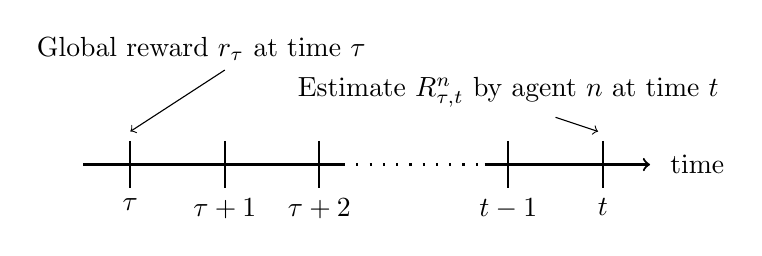
\begin{tikzpicture}[scale=0.6] % Smaller scale

    % Timeline with arrow
    \draw[black,thick, -] (-2.5,0) -- (3,0);
    \draw[black,thick, ->] (6,0) -- (9.5,0); % Horizontal line with arrow at the end

    % Markers with labels
    \draw[thick,black] (-1.5,0.5) -- (-1.5,-0.5) node[below] {$\tau$};
    \draw[thick,black] (0.5,0.5) -- (0.5,-0.5) node[below] {$\tau+1$};
    \draw[thick,black] (2.5,0.5) -- (2.5,-0.5) node[below] {$\tau+2$};

    % Dotted line for the break between $\tau+2$ and $T-1$
    \draw[loosely dotted,thick,black] (3,0) -- (6,0); % Dotted line between tau+2 and T-1

    % More markers and labels
    \draw[thick,black] (6.5,0.5) -- (6.5,-0.5) node[below] {$t-1$};
    \draw[thick,black] (8.5,0.5) -- (8.5,-0.5) node[below] {$t$};


    \node[above] at (0,2) {Global reward $r_\tau$ at time $\tau $};
    \draw[->] (0.5,2) -- (-1.5,0.7) ;

    % Agent n above T
    \node[above] at (6.5,1) {Estimate $R^n_{\tau,t}$ by agent $n$ at time $t$};
    \draw[->] (7.5,1) -- (8.4,0.7) ;

    % Arrow pointing to the end, with label t
    \node at (10.5,0) {time}; % Label 'time' at the end
    %\draw[thick, ->] (9, 0) -- (9.5, 0); % Arrow pointing to the right to indicate end
    
\end{tikzpicture}

    \caption{\emph{Gossip} timeline: Each agent aims to estimate the global vector of rewards $r(S_{\tau})$. After $t-\tau$ time steps, the local estimation of $r(S_{\tau})$ obtained by agent $n$ is $R_{\tau,t}^n$.}
    \label{fig:timeline} 
\end{figure}
%
Consider an agent $n^\prime$ whose state $S_\tau^{n^\prime}$ is in region $\mathcal S_m$  at time $\tau$. That is $S_\tau^{n^\prime}\in \mathcal S_m$ as shown in Figure~\ref{fig:gossip_stochastic} for the case of our monitoring Example \ref{example}. Then agent $n^\prime$ knows first-hand that the reward for the region $S_m$ is being attended at this specific time $\tau$, and thus the global reward $(r(S_{\tau}))_m = 1$ is being attained. Hence, it sets its own local estimate of the reward to one,  i.e., $(R_{\tau,t}^{n^\prime})_m = (r(S_{\tau}))_m = 1 \ \textrm{for all}\ t\geq \tau$. Then, it passes this information to its neighbors, who will update their local estimates of the reward $(r(S_{\tau}))_m$ accordingly. Specifically, each agent will receive the local estimates of $r(S_{\tau})$ from its neighbors and set its local estimate to $1$ if any of its neighbors have a local estimate of $1$ for the same region. That is equivalent to using the maximum of the local estimates of its neighbors, including itself. In general, the update rule for the local copies of the rewards is given by
%
\begin{align}\label{eqn_gossip_r}
    	\left(R_{\tau,t}^n\right)_m&=\begin{cases}
    	\textcolor{black}{\max_{n^\prime\in\mathcal N_n\cup \{n\}} \left(R_{\tau,t-1}^{n^\prime}\right)_m},& t>\tau\\
    	\mathds 1\{S_{t}^n\in\mathcal S_m\},& t=\tau,
    	\end{cases}
\end{align}
%
where $\mathcal N_n$ is the (stochastic, time-varying) neighborhood of agent $n$ at time $t$, and $\mathds 1\{S_{t}^n\in\mathcal S_m\}$ is the direct observation that the state of agent $n$ is in $\mathcal S_m$ at time $t$. During each rollout $k$, agent $n$ keeps the series of estimates $R_{\tau,t}^{n},\ \tau=kT_0,\ldots,(k+1)T_0-1 $, updating them recursively via \eqref{eqn_gossip_r} at each time $t=\tau,\ldots,(k+1)T_0-1$.

Using these \emph{gossiped} reward estimates to update the multipliers, the distributed version of \eqref{eqn_contractive_big_brother} becomes
%
\begin{align}\label{eqn_stochastic_dual}
    \lambda_{k+1}^n = \left[(1-\alpha) \lambda_k^n + \frac{\eta}{T_0} \sum_{\tau=k T_0}^{(k+1) T_0-1}\left(c-R_{\tau,(k+1)T_0-1}^n \right)\right]_{+}
\end{align}
%
where agent $n$ waits as much as possible until the end of the rollout at time $t=(k+1)T_0-1$ to substitute $R_{\tau,(k+1)T_0-1)}$ for $r(S_{\tau})$ and thus have the best possible estimate.  

Equations \eqref{eqn_gossip_r} and \eqref{eqn_stochastic_dual}, together with the policy structure in \eqref{eqn_separate_policy},  are the main tools for the distributed implementation of the dual update, allowing agents to run the fully distributed policy in Algorithm \ref{algo:alg_main_algorithm}.

\begin{algorithm}[t]
\caption{Distributed multi-agent  policy execution}\label{algo:alg_main_algorithm}
\begin{algorithmic}[1]
\FOR{$k=0,1,\ldots$}
  \STATE Substitute $\lambda^{k}_n$ in \eqref{eqn_optimal_trained_policy}  pretrained with local gradients.
  \STATE Keep the local realizable policy $\pi_{\theta^n}[\lambda^{k}_n]$ as in \eqref{eqn_realizable_policy}.
  \FOR{$t=k T_0,\ldots,(k+1)T_0-1$}
  	\STATE Act $A^n_t\sim \pi_{\theta^n}[\lambda^{k}_n]$ and transition to $S_{t+1}^n$.\\
    \STATE Collect local rewards $(R_{t,t}^n)_m=\mathds{1}\{S_t^n\in\mathcal S_m\}$. \\
  	\STATE \emph{Network gossiping:} Update $ R_{\tau,t}^n$ as in \eqref{eqn_gossip_r}.
  \ENDFOR
   \STATE Update the multipliers according to \eqref{eqn_stochastic_dual}.
\ENDFOR
\end{algorithmic}
\end{algorithm}

In executing Algorithm \ref{algo:alg_main_algorithm}, agents use a \emph{realizable} policy $\pi_{\theta}[\lambda^1,\ldots,\lambda^N]$ in the sense that it is parametric, trained with finite rollouts as in \eqref{eqn_optimal_trained_policy}, and with local copies of the multipliers. Specifically, each agent $n$ substitutes its local copy of the vector of multipliers $\lambda^n$ for $\lambda$ in \eqref{eqn_separate_policy} to obtain  its local part of the realizable policy  $\pi_{\theta^n}(A_t^n\mid S_t^n,\lambda^n)$. Accordingly, the realizable global policy corresponds to  their product
%
\begin{align}\label{eqn_realizable_policy}
\pi_\theta[\lambda^1,\ldots,\lambda^N](A_t\mid S_t)&:=\prod_{n=1}^N\pi_{\theta^n}(A_t^n|S_t^n,\lambda^n).
\end{align}

By using the  distributed policies in \eqref{eqn_realizable_policy}, the team achieves the following realizable value
\begin{align}\label{eq:non-idealities-VR}
V_R&:=V_{T_0}\left(\pi_\theta[\lambda_k^1 \ldots \lambda^N]\right)
=\mathbb E_{\pi_\theta}\left[\frac{1}{T_0} \sum_{t=k T_0}^{(K+1) T_0-1} r(S_t)\ \right].
\end{align}

Because agents cannot guarantee to reach exact consensus on the multipliers $\lambda^n$ almost surely when communicating over the stochastic graph \eqref{eqn_graph_model}, their realizable policies $\pi_{\theta^n}(\lambda^n)$ will differ from the one $\pi_{\theta^n}(\lambda)$ trained for, which assumed global access to $\lambda$. To mitigate the effect of this mismatch, we need the following assumption. 

\begin{assumption}[Lipschitz continuity of value functions]\label{assumption:lipschitz}
The difference between the value functions $V_P$ and $V_R$ with global and distributed multipliers, as defined in \eqref{eq:non-idealities-VP} and \eqref{eq:non-idealities-VR}, respectively, is bounded by the scaled difference  their multipliers with scaling constant $L>0$, i.e., 
\begin{align}
\nonumber \|V_P-V_R\|&=\|V_{T_0}(\pi_\theta[\lambda, \ldots, \lambda]) - V_{T_0}(\pi_\theta[\lambda^1, \ldots, \lambda^N])\|\\& \leq L \max_{n=1,\ldots,N}\|\lambda - \lambda^n\|_\infty.
\end{align} 
\end{assumption}

This assumption requires the parametric policies in \eqref{eqn_optimal_trained_policy} to be Lipschitz with respect to the multipliers, which is the case, for instance, if we choose neural networks for the policy parameterization with bounded weights and Lipschitz activation functions such as ReLU. 

To quantify such an error, we measure the probability that the true rewards reach all agents. Referring back to Figures~\ref{fig:gossip_stochastic} and \ref{fig:timeline}, the event that at time $t$ agent $n$ knows whether there is an agent $n^\prime$ that satisfied $S_t^{n^\prime}\in \mathcal S_m$ at a previous time $\tau$  is given by $(R_{\tau,T}^n)_m = (r(S_{\tau}))_m$. The distribution of that event follows a negative binomial distribution, as is stated in the following proposition. 

\begin{proposition} \label{prop_binomial}
    Given the Bernoulli graph model \eqref{eqn_graph_model}, the probability that agent $n$ knows the global reward $r(S_{\tau})$  at time $t\geq \tau$ is
    $$\mathbb P\left((R_{\tau,t}^n)_m = (r(S_{\tau}))_m\right)\leq \mathbb P\left(BN(d_G, p)\leq t-\tau\right),$$
    where $d_G$ is the diameter of the underlying graph $G$, $p$ is the probability that an edge of the graph is active, and $BN(d_G,p)$ denotes the negative binomial distribution.
\end{proposition}
\begin{proof}
     See Appendix \ref{app:proof_prop_binomial}.
\end{proof}
%
Leveraging Proposition \ref{prop_binomial}, the following result  provides a bound for the multipliers' error.
%
\begin{proposition}\label{prop_gossip_error}
       Given the Bernoulli graph model \eqref{eqn_graph_model}, the  error norm between multipliers $\lambda_k$ and $\lambda_k^n$ in \eqref{eqn_contractive_big_brother} and \eqref{eqn_stochastic_dual}, computed in terms of the rewards $r(S_\tau)$ and their estimators $R_{\tau,t}^n$, respectively is bounded by
       %
\begin{align}\label{eq:lambdadif}\mathbb 
E\left[ \|\lambda_k^n-\lambda_k\|_\infty \right]\leq \frac{\eta d_G}{\alpha T_0 p},
\end{align}
where $d_G$ is the diameter of the underlying graph $G$, and $p$ is the probability that an edge of the graph is active.
\end{proposition}
 \begin{proof}
     See Appendix \ref{app:proof_prop_gossip_error}.
 \end{proof}
 
{According to \eqref{eq:lambdadif}, the error between the global and local multipliers is controlled by the step size $\eta$, the contraction parameter $\alpha$, and the rollout horizon  $T_0$.  
The trade-off for choosing $T_0$  entails keeping the truncation error $\epsilon$ in Assumption \ref{assumption_representation} sufficiently small and reducing the multipliers' error while ensuring that the multipliers are updated sufficiently often in order to speed training and increase the agents' agility in the online phase. Reducing $\eta$ also reduces the bound in \eqref{eq:lambdadif} at the expense of a slower dual update and policy reaction. %The contraction factor $\alpha$ can also used to control the multiplier error resulting from using $R_{t,(k+1)T_0}^n$ instead of $r(S_t)$, but it has a negative effect in the feasibility guarantees, as we will establish in the next section.
}%blue
%\textcolor{red}{sluggish policy means not clear?}
%\santiago{The previous text should discuss the result of the proposition. And tie it better with the remark.}

\begin{remark}
    Proposition \ref{prop_gossip_error} also demonstrates the role of $\alpha$.  Including the contraction factor $(1-\alpha)$ in the dual update is key to guarantee that the deviation of the distributed multipliers remains bounded. Indeed, as the recursive addition of rewards accumulates over successive rollouts, the reward errors need to be modulated by powers of $(1-\alpha)$ to ensure that their aggregate effect in \eqref{eq:lambdadif} is subdued. A higher $\alpha$ makes the dual update more contractive, resulting in a smaller error in \eqref{eq:lambdadif}. However, increasing $\alpha$ has an adverse effect on the feasibility guarantees, as we will establish in the next section.
    %blue
\end{remark}
%




 \section{Feasibility Analysis}\label{sec:feasibility}
 
In this section we present the main result of our work which is to guarantee that the trajectories generated by Algorithm \ref{algo:alg_main_algorithm} are almost surely feasible in the sense that the time-averaged rewards exceed thresholds $c$, within an error controlled by the parameter $\alpha$, with probability one.

\subsection{Main Result}\label{ssec_main_result} 

Before stating the feasibility guarantees we require an additional assumption regarding the underlying MDP.

\begin{assumption}\label{assumption_noforces}(No repelling forces).
\textcolor{black}{The underlying Markov decision process is such that, given $m$, there exists a policy  structured as in  \eqref{eqn_ideal_separated_policy} which satisfies $\left(r(S_t)\right)_m=1$ for all $t$.}
\end{assumption}

This assumption implies that, if necessary, an agent can keep its state stationed in a particular region $S_{t}^n\in \mathcal S_m$. We added this assumption for simplicity to attain $(V)_m=1$ and make the constraint $m$  feasible with a margin  $1-(c)_m$.
Assumption \ref{assumption_noforces} can be substituted by a more general version $(V)_m\geq c>(c)_m$, only affecting the parameter $\delta$ in the following Theorem \ref{theorem:feasibility}. This milder version would hold, for instance, if $S_{t}^n\in \mathcal S_m$ is attainable a fraction of time $c\leq 1$.

We are now in conditions to state our main result.

\begin{theorem}\label{theorem:feasibility}
Let Assumptions \ref{assumption_representation}--\ref{assumption_noforces} hold, and consider the specifications $\|c\|_\infty <1$,  and $\|c\|_1 \leq N-1$. If 
\begin{align}\label{eq:delta_theorem}
\delta:=\left(1-\|c\|_\infty\right) - M\left(\epsilon+\beta\right)>0,
\end{align} 
%
the trajectories generated by Algorithm \ref{algo:alg_main_algorithm} over the stochastic  communication network \eqref{eqn_graph_model}  are feasible within an error  $\sqrt{\alpha M}$ with probability one, i.e.

\begin{equation}\label{eqn_as_feasibility}
    \liminf_{T\to \infty}\frac{1}{T} \sum_{t=0}^{T-1}  r(S_t)\geq c - \mathbf  1 \sqrt{\alpha M}, \mbox{ a.s.}
    \end{equation} %blue
with $\mathbf 1$ being the vector of all ones and 
\begin{equation}\label{eq:alpha_bound}
    \alpha\geq\frac{\eta d_G}{p T_0}  \frac{M L}{\delta}.
\end{equation}
\end{theorem}
\begin{proof}
    See Section \ref{ssec:proof_th}.
\end{proof}

Since the constraints  \eqref{eqn_crl} involve time averages of binary rewards, the thresholds in $c$ must be no larger than one for a feasible policy to exist. Theorem \ref{theorem:feasibility} imposes a stricter requirement $\|c\|_\infty <1$, %, such that all thresholds in the vector $c$ are strictly less than one, 
leaving a margin for the realizable policies.  Also  $\|c\|_1 \leq N-1$ is imposed, ensuring that $N-1$ agents can satisfy all constraints with a margin for the transients when agents' states cycle around regions $\mathcal S_m$. Additionally, condition \eqref{eq:delta_theorem} %requires not only $\|c\|_\infty <1$ but also 
imposes limits on the approximation error in training, with $\beta$ and $\epsilon$ being the quantities defined in Assumption \ref{assumption_representation}.%eqthat the parameterization is sufficiently expressive and the horizon $T_0$ sufficiently large to make $\beta + \epsilon$ small enough.  

The result in Theorem guarantees that we can attain almost sure feasibility of a surrogate problem \eqref{eqn_crl} where we tighten the constraints by increasing the thresholds to leave a margin for the error $\sqrt{\alpha M}$ in \eqref{eqn_as_feasibility}, and we run Algorithms \ref{alg:offline} and \ref{algo:alg_main_algorithm} using these surrogate thresholds. The value of $\alpha$ in \eqref{eq:alpha_bound} can be made arbitrarily small by designing a rich parameterization or neural network, a long time horizon $T_0$, and a small step size $\eta$. These parameters introduce a trade-off between reducing the error and slowing training.

The result in Theorem \ref{theorem:feasibility} is derived by unrolling the stochastic dual recursion in \eqref{eqn_stochastic_dual} to write the sum of the rewards in terms of the multipliers, which yields an expression for the feasibility error in terms of the stochastic average of the multipliers along a trajectory. 
Hence, the proof is completed by bounding this stochastic average by $\eta \sqrt{M/\alpha}$. 
%
To obtain this bound for the stochastic average, we utilize proof techniques similar to those in stochastic gradient descent on the dual domain,
 for which it is key to show that the gradient of the dual forms an acute angle with the vector of multipliers, i.e.    
\begin{align}
\lambda^\top (V-c)&\geq 0.\label{eqn_accute_angle}
\end{align}

In this direction, Lemma \ref{lemma:positive_ideal_value} below indicates that if we use the ideal policy $\pi^\star[\lambda,\ldots,\lambda]$ in \eqref{eqn_optimal_set}, the condition  \eqref{eqn_accute_angle} is satisfied even with a slack  $(1-\|c\|_{\infty})\|\lambda\|/\sqrt{M}$, that will become handy when considering the realizable policy in \eqref{eq:non-idealities-VR} instead.  The proof of Lemma \ref{lemma:positive_ideal_value} uses Assumption \ref{assumption_noforces} to ensure that the underlying MDP does not prevent the agents from taking care of the most pressing constraints. The value $V$ in \eqref{eqn_ideal_V} and \eqref{eqn_accute_angle} assumes that we could train with infinite horizon, without the limitations of parametrization, and with all agents having access to the same  multipliers in \eqref{eqn_contractive_big_brother}. On the other end, $V_R$ in \eqref{eq:non-idealities-VR} corresponds to the  realizable policy in Algorithm \ref{algo:alg_main_algorithm},  and is obtained by  applying  the distributed, finite horizon  and parametric procedures behind equations \eqref{eqn_optimal_trained_policy} and \eqref{eqn_stochastic_dual}. In particular, each agent utilizes its own copy of local multipliers in \eqref{eqn_stochastic_dual}. In between $V$ and $V_R$, we defined  $V_P$ in \eqref{eq:non-idealities-VP} as a theoretical value to be used as an intermediate step in the proofs of feasibility. It differs from $V$ in using a parametric policy and in aggregating the rewards for a finite time period of length $T_0$. And $V_P$ is different from $V_R$ in assuming global access by all agents to the same multipliers. We use Assumptions \ref{assumption_representation} and \ref{assumption:lipschitz} in Lemma \ref{lemma:error_gradient} to bound the difference $\lambda^\top(V-V_R)$. If this difference is lower than the slack $(1-\|c\|_{\infty})\|\lambda\|/\sqrt{M}$, then \eqref{eqn_accute_angle} will still be satisfied if we substitute  $V_R$ for $V$. 

\subsection{Proof of Theorem \ref{theorem:feasibility} and Supporting Results}\label{ssec:proof_th}

We proceed to prove our first result. The intuition in Lemma \ref{lemma:positive_ideal_value} is that if we fix $\lambda$, the ideal optimal policy assigns the $N$ agents to the regions $\mathcal S_m$ with highest weighted rewards. As the multipliers cycle in the execution phase according to Algorithm \ref{algo:alg_main_algorithm}, this ideal behavior will drive the agents to cyclically attend the most pressing constraints at each rollout.   

\begin{lemma}\label{lemma:positive_ideal_value}
Assumption \ref{assumption_noforces} with $\|c\|_{\infty}<1$ and $\|c\|_1 \leq N-1$  as in Theorem \ref{theorem:feasibility} results in
 %
 \begin{align}\lambda^\top (V-c)&\geq (1-\|c\|_{\infty})\frac{\|\lambda\|}{\sqrt{M}}.\label{eqn_lemma_vI}
 \end{align}
 \end{lemma}
%
\begin{proof}
Without loss of generality, sort the multipliers $\left(\lambda\right)_1\geq \left(\lambda\right)_2\geq\cdots\geq \left(\lambda\right)_M$, so that $\left(\lambda\right)_1$ is the largest multiplier.

One policy that optimizes the Lagrangian would assign an agent to each region $\mathcal S_m$ of the state space for $m=1\ldots,N$, since there are only $N<M$ agents. Therefore, $\left(V\right)_m=1$ for $m\leq N$ and $\left(V\right)_m=0$ for $m>N$. Hence it follows that
%
\begin{align}\label{eq:inner_product_decomposition}
\lambda^\top (V-c) &= \left(\lambda\right)_1 (1-\left(c\right)_1) \\
&+ \sum_{m=2}^N \left(\lambda\right)_m (1-\left(c\right)_m) 
+\hspace{-9pt}\sum_{m=N+1}^M\hspace{-5pt}\left(\lambda\right)_m (0-\left(c\right)_m). \notag
\end{align}

Next, we use the fact that $\left(c\right)_1 \leq \|c\|_{\infty}$ by definition of the infinity norm, so that $(1-(c)_1)\leq (1-\|c\|_\infty)$. Also, the multipliers were sorted in decreasing order which implies that the first one is maximum $(\lambda)_1=\| \lambda\|_\infty$, the following  $N-1$  satisfy $ (\lambda)_m\geq (\lambda)_N$ for all $2\leq m\leq N$, and the last $M-N$ satisfy $(\lambda)_m\leq (\lambda)_N$ for all $m>N$. Hence, we bound the three terms in  \eqref{eq:inner_product_decomposition} by
\begin{align}
\lambda^\top (V-c) &\geq (1-\|c\|_{\infty}) \|\lambda\|_\infty\\ &+(\lambda)_N  \sum_{m=2}^N (1-\left(c\right)_m)
-(\lambda)_N  \sum_{m=N+1}^M \left(c\right)_m\nonumber\\
%&=(1-\|c\|_{\infty}) \|\lambda\|_{\infty} +(\lambda)_N \left((N-1) - \sum_{m=2}^M \left(c\right)_m\right)\\
&\geq (1-\|c\|_{\infty}) \|\lambda\|_{\infty} +(\lambda)_N \left((N-1) - \|c\|_1\right), \nonumber
\end{align}
%
where we grouped the terms multiplying $\lambda_N$ and then used $\|c\|_1=\sum_{m=1}^M (c)_m\geq \sum_{m=2}^M (c)_m$. Given that  $(N-1) \geq \|c\|_1$ by hypothesis, we can write
%
\begin{align}
\lambda^\top (V-c) &\geq (1-\|c\|_{\infty}) \|\lambda\|_{\infty}. 
\end{align}
%
Then use the property $\|\lambda\|_{\infty} \geq \|\lambda\|/\sqrt{M}$.
\end{proof}

The following results bounds the error incurred in executing the realizable policy \eqref{eqn_realizable_policy} as compared to the ideal policy \eqref{eqn_ideal_separated_policy}. Intuitively, Lemma \ref{lemma:error_gradient} guarantees that when agents use the realizable policy, they still behave as in the ideal case of  Lemma \ref{lemma:positive_ideal_value}, attending the most pressing constraints during the current rollout. Its proof uses Assumption  \ref{assumption_representation} to bound the error between $V$ and $V_P$, and Assumption \ref{assumption:lipschitz} together with Proposition \ref{prop_gossip_error} for the error between $V_P$ and $V_R$. 

\begin{lemma}\label{lemma:error_gradient}
Given the stochastic communication network model \eqref{eqn_graph_model}, 
Assumptions \ref{assumption_representation}--\ref{assumption:lipschitz} ensure that the following bound holds for the difference between the gradient of the ideal and realizable value functions %
\begin{align}  (\lambda_k)^\top \left(V-V_R\right)\leq \|\lambda_k\|\left(\epsilon+\beta+\eta L \sqrt{M} \frac{d_G}{\alpha T_0 p}\right),\label{eqn_lemma_Error_VI_VR}
\end{align}
%
where $V$ and $V_R$ are defined in \eqref{eqn_ideal_V} and \eqref{eq:non-idealities-VR}.
\end{lemma}
\begin{proof}

Write the norm of the difference between the ideal and realizable value functions as
$
    \left\|V_R-V\right\| \leq\left\|V-V_P\right\|+\left\|V_P-V_R\right\|,
$
%
using the triangle inequality and summing and subtracting the term $V_P$. Hence, by  Assumptions \ref{assumption_representation} and \ref{assumption:lipschitz} 
\begin{equation}
\left\|V_R-V\right\| \leq \epsilon+\beta+L \max_{n=1,\ldots,N} \left\|\lambda_k^n-\lambda_k\right\|_\infty,
\end{equation}
and lastly, using Proposition \ref{prop_gossip_error}, we obtain

$\left\|V_R-V\right\| \leq \epsilon+\beta+L \epsilon_G=\epsilon+\beta+\eta L \sqrt{M} d_G/(\alpha T_0 p).$
\end{proof}
%

Combining Lemmas \ref{lemma:positive_ideal_value} and  \ref{lemma:error_gradient}, if conditions \eqref{eq:delta_theorem} and \eqref{eq:alpha_bound} in Theorem \ref{theorem:feasibility} are satisfied, then \eqref{eqn_accute_angle} holds for the realizable policy and $V_R$. Indeed, from \eqref{eqn_lemma_vI} and \eqref{eqn_lemma_Error_VI_VR}  it yields 
\begin{align}
&\lambda^\top (V_R-c) = \lambda^\top(V-c) + \lambda^\top (V_R-V)\label{eqn_real_accute}\\
&\geq\frac{\|\lambda\|}{\sqrt{M}}\left((1-\|c\|_\infty)-M\left(\beta+\epsilon +\eta L  \frac{d_G}{\alpha T_0 p}\right)\right)\geq 0 ,  \nonumber 
\end{align}
where the last inequality requires $\delta>0$ in \eqref{eq:delta_theorem} and it is equivalent to $\alpha \geq {\eta d_G M L}/(p T_0 \delta )$ in \eqref{eq:alpha_bound}.

Having a positive inner product in \eqref{eqn_real_accute}, we can prove that the stochastic average of the multipliers across a trajectory is bounded.  
%
This key result is presented below as Proposition \ref{proposition:combined_lemma}.  Its proof,  relies on three steps. First, we combine \eqref{eqn_real_accute} with the update \eqref{eqn_contractive_big_brother} to obtain a contractive system with constant input for the expected value of $\|\lambda\|$ conditioned on past values. From this contraction, it follows that the expected value of the time average of the multipliers is bounded. Lastly, we include a modified proof of the strong law of large numbers for non-i.i.d. variables, which lets us drop the expected value and reach the following result.

\begin{proposition}
\label{proposition:combined_lemma}
Given the  stochastic  communication network model \eqref{eqn_graph_model}, under Assumptions \ref{assumption_representation}--\ref{assumption_noforces}, and with $\|c\|_\infty<1$, $ \|c\|_1\leq N-1$,
$\delta=\left(1-\|c\|_\infty\right) - \sqrt{M}\left(\epsilon+\beta\right)>0,$ and $\alpha\geq\frac{\eta d_G}{p T_0} \cdot \frac{\sqrt{M} L}{\delta}$, the averaged rewards along a trajectory are bounded by $\eta \sqrt{M/\alpha}$ with probability $1$, i.e.,
\begin{align}\label{eqn_bound_stochasstic_average}
\limsup_{k \rightarrow \infty} \frac{1}{k} \sum_{i=1}^{k} \left(\lambda_i\right)_m \leq \eta \sqrt{\frac{ M}{\alpha}} \text { a.s.. }
\end{align}
\end{proposition}
\begin{proof}
See Appendix \ref{app:combined_lemma}.
\end{proof}

\begin{figure*}[t!]
   \centering
   \begin{subfigure}{0.65\columnwidth}
   		\centering
            \begin{figure*}
\begin{center}
\includegraphics[width=\linewidth]{figs/src/navigation.pdf}
\vspace{-15pt}
\caption{\textbf{Realworld Orientation-Aware Navigation.} We present both the third-person view and the egocentric view, annotating the predicted orientation of the interacted objects.}
\label{fig:navigation}
\end{center}
\end{figure*}
   		\caption{Floor plan.}	
            \label{fig:floorplan}
   \end{subfigure}
   \begin{subfigure}{0.65\columnwidth}
   		\centering
\input{./figs/heatmap_agent0_floorplan}
   		\caption{Agent $0$.}
   		\label{fig:heatmap_agent0}
   \end{subfigure}
   \begin{subfigure}{0.65\columnwidth}
   		\centering
\begin{tikzpicture}[scale=0.18]
\pgfplotsset{grid style={loosely dashed,gray!50,line width=2pt}}
\begin{axis}[
   xmin=0, xmax=30,
    ymin=0, ymax=14,
    width=30cm, height=14cm,
    ticklabel style = {font=\huge},
    ytick={0,2,4,6,8,10,12,14},
    xtick={0,2,4,6,8,10,12,14,16,18,20,22,24,26,28,30},
    grid=both,
    %enlarge	limits=false,
    colormap/cool,
    colorbar,
    point meta min=0,
    point meta max=9,
    scatter src=explicit,
%    colormap={custom}{
%        rgb255=(255,255,255)   % White
%        rgb255=(255,255,0)     % Yellow
%        rgb255=(255,0,0)       % Red
%        rgb255=(0,0,0)       % Black
%    },
     %colormap={slategraywhite}{rgb255=(255,255,255) rgb255=(255,0,0)},
]

	\addplot+[only marks, scatter, mark=*, mark size=6pt, opacity=0.9, scatter/use mapped color={draw opacity=0,fill=mapped color}] table[x index=0, y index=1, meta index=3] {figs/data/heatmap_agent1.dat};

    % room0
    \addplot[draw=black, line width=4pt] coordinates {
      (0,0) (10,0) (10,12) (0,12) (0,0)};
    %room 1
    \addplot[draw=black, line width=4pt] coordinates {
       (10,0) (10,12) (15,12) (15,0)(10,0)};
    
    %room 2
    \addplot[draw=black, line width=4pt] coordinates {
       (15,0) (15,12) (24,12) (24,5)(26,5) (26,0) (15,0)};
   
	%room 3
    \addplot[draw=black, line width=4pt] coordinates {
       (26,10.9) (26,14) (30,14) (30,10)(26,10)(26,10.1)};
	%door room room 3
   	%\addplot[draw=black!25!white ] coordinates { (26,10.1) (26,10.9)};

	%room 4
    \addplot[draw=black, line width=4pt] coordinates {
       (26,6.9) (26,10) (30,10) (30,6)(26,6)(26,6.1)};

	%door room 4
  	% \addplot[draw=black!10!white  ] coordinates { (26,6.1) (26,6.9)};
	%room 5
    \addplot[draw=black, line width=4pt] coordinates {
        (26,5.9)(26,6) (30,6) (30,0)(26,0)(26,5.1)};
	%door room 5
 	%\addplot[draw=black!25!white  ] coordinates { (26, 5.1) (26, 5.9)};


	%door room 0 - left
    \addplot[draw=white, line width=5pt] coordinates {(1.6,12) (2.4,12)};
    %door room 0 - right
    \addplot[draw=white, line width=5pt] coordinates {(8.6,12) (9.4,12)};
	%door room 1
    \addplot[draw=white, line width=5pt] coordinates {(13.6,12) (14.4,12)};
	%door room 2 upper
    \addplot[draw=white, line width=5pt] coordinates {(15.6,12) (16.4,12)};
	%door 2 lower
    \addplot[draw=white, line width=5pt] coordinates {(24.6,5) (25.4,5)};

    %zone 0
	\draw [opacity=0.75, draw=red, thick, fill=red!75] (axis cs:6,9) circle [radius=1];
	%zone 1
    \draw [opacity=0.75, draw=green, thick, fill=green!75] (axis cs:13,9) circle [radius=1];
	%zone 2
    \draw [opacity=0.75, draw=blue, thick, fill=blue!75] (axis cs:20,9) circle [radius=1];
	%zone 3
    \draw [opacity=0.75, draw=orange, thick, fill=orange!75] (axis cs:28,12) circle [radius=1];
	%zone 4
    \draw [opacity=0.75, draw=cyan, thick, fill=cyan!75] (axis cs:28,8) circle [radius=1];
	%zone 5
    \draw [opacity=0.75, draw=magenta, thick, fill=magenta!75] (axis cs:28,4) circle [radius=1];

	%floorplan rectangle
    \addplot[draw=black, line width=4pt] coordinates {(0,0) (0,14) (30,14) (30,0)(0,0)};
      
\end{axis}
\end{tikzpicture}     
   		\caption{Agent $1$.}
   		\label{fig:heatmap_agent1}
   \end{subfigure}   \\
   \begin{subfigure}{0.65\columnwidth}
   		\centering
\input{./figs/heatmap_agent2_floorplan}       		
            \caption{Agent $2$.}
   		\label{fig:heatmap_agent2}
   \end{subfigure}   
     \begin{subfigure}{0.65\columnwidth}
   		\centering
\input{./figs/heatmap_agent3_floorplan}
   		\caption{Agent $3$.}
   		\label{fig:heatmap_agent3}
   \end{subfigure}
   \begin{subfigure}{0.65\columnwidth}
   		\centering
\input{./figs/heatmap_agent4_floorplan}     
   		\caption{Agent $4$.}
   		\label{fig:heatmap_agent1}
   \end{subfigure}   
\caption{(a) Floor plan and sample trajectories for each of the $N=5$ agents, $n=0,\ldots,4$. Black lines represent walls, and colored circles represent the $M=6$ zones to be patrolled by the agents. Each colored dot along a trajectory indicates a new position for each time step. The $12$ gray rectangular regions define distinct possible tiles or observations of an agent’s position, which are the inputs to the policy. Figures (b)--(f): Occupation heat maps. The complete trajectory of an agent across $40{,}000$ timesteps is represented by dots, indicating the position reached by an agent. Each dot color represents the frequency of occupation at that position, with darker hues indicating more frequent positions, under a logarithmic colorbar scale.}
\label{fig:heatmaps}
\end{figure*}

Hence, we proceed with the proof of  Theorem \ref{theorem:feasibility}. It yields from applying the results of Proposition \ref{proposition:combined_lemma} to the update rule \eqref{eqn_contractive_big_brother}.  Specifically, we introduce
\begin{equation}
    \bar r_k^{T_0}=\frac{1}{T_0}\sum_{\tau=(k-1)T_0}^{kT_0-1}r(S_t),
\end{equation}
which  reduces notation and lets us rewrite the update \eqref{eqn_contractive_big_brother} as
\begin{align}\label{eq:proyection_inequality}
    \lambda_{k+1}&=\left[(1-\alpha) \lambda_k+\eta\left(c-\bar r_k^{T_0}\right)\right]_{+}\\
    &\geq (1-\alpha)\lambda_k+\eta\left(c-\bar r_k^{T_0}\right), \notag
\end{align}
where the inequality that arises from the projection must be understood component-wise. Thus, from \eqref{eq:proyection_inequality}, we can rewrite
\begin{align}&
\eta\left(\bar r_k^{T_0}-c\right) \geq  (1-\alpha) \lambda_k -\lambda_{k+1}.
\end{align}

Hence, assuming $\lambda_0=0$, adding over $k=0,\ldots,K$
\begin{align}\label{eq:constraint_lambda}
&\sum_{k=0}^K \eta\left(\bar r_k^{T_0}-c\right) \geq \sum_{k=0}^K(1-\alpha) \lambda_k-\sum_{k=0}^K\lambda_{k+1} \\
&
= \sum_{k=1}^K(1-\alpha)  \lambda_k  -\sum_{k=1}^{K} \lambda_{k} -\lambda_{K+1} 
= -\sum_{k=1}^K\alpha  \lambda_k   -\lambda_{K+1}, \nonumber 
\end{align}
where we removed the term corresponding to $\lambda_0$, substituted $k=k+1$ in the sum of $\lambda_{k+1}$ and then rearranged two sums into one removing those terms $\lambda_k$ that cancel each other. Moving $c$ and $\eta$ to the right-hand side, we further obtain
\begin{align}
    & \frac{1}{K} \sum_{k=0}^K  \bar r_k^{T_0}\geq c -  \frac{1}{\eta K} \lambda_{K+1}  - \frac{\alpha}{\eta}\frac{1}{K} \sum_{k=1}^{K}   \lambda_k, \label{eq:constraint_with_lambdaK}
\end{align}
%
and using Proposition \ref{proposition:combined_lemma}, results in
%
\begin{align}& \liminf_{K\to\infty}\frac{1}{K} \sum_{k=1}^K  \bar r_k^{T_0}\geq c-\alpha\sqrt{\frac{ M}{\alpha}}.  \label{eq:constraint_satisfaction_mean}
\end{align}

We demonstrated throughout this section that selecting $\alpha>0$, which is required according to Proposition \ref{prop_gossip_error} to ensure that the multiplier error remains bounded, introduces an error in the feasibility result \eqref{eqn_as_feasibility}. Thus, we want to make $\alpha$ as small as possible, but this is limited by \eqref{eq:alpha_bound}, which is imposed to ensure the dual descends according to  \eqref{eqn_real_accute}. We can adjust $\eta$ and $T_0$ and $p$ to reduce the lower bound for $\alpha$ in \eqref{eq:alpha_bound}. In particular, the activation probability $p$ in the stochastic communication graph depends on the communication scheme that is part of the problem design. In the next section, we provide an example of how to increase this probability by boosting the communication power.  


\section{Numerical Experiments}\label{sec_numerical}
  
In the following, we present numerical experiments designed to test the performance of the proposed multi-agent reinforcement learning Algorithm \ref{algo:alg_main_algorithm}. We consider a scenario with five robots acting as agents, which navigate and monitor  multiple rooms in a floor plan.
    
\subsection{Floor Plan Navigation}

Consider $N=5$ agents navigating a floor plan of an L-shaped corridor connecting three offices and three laboratories at the University of Pittsburgh, with their separating walls represented as black lines (see Fig. \ref{fig:heatmaps}). In this scenario, the state of agent $n$ at time $t$ is $S^n_t=(x^n_t,y^n_t)$  with $x^n_t$ and $y^n_t$ representing the agent horizontal and vertical coordinates, respectively with $S^n_t \in [0,30]\times[0,14]$, all measured in meters. Correspondingly, the $M=6$ regions    $\mathcal S_1,\ldots,\mathcal S_M$ are depicted by the colored circles in Fig. \ref{fig:heatmaps}, centered at $(x_1,y_1)=(6,9)$, $(x_2,y_2)=(13,9)$, $(x_2,y_2)=(20,9)$, $(x_3,y_3)=(28,4)$, $(x_4,y_4)=(28,8)$, and $(x_5,y_5)=(28,12)$, and with all  radius equal to one. The global reward corresponding to zone $m$ takes the value $(r(S_t))_m=1$ if at least one agent enters the corresponding circle. The action space $\mathcal A=\{0,\ldots,5\}$ is finite, meaning that the agents must decide  which of the six regions to visit at each instant. We assume a low-level robot  navigation control is available to drive the agent across the floor plan toward the selected zone. This controller follows a sequence of segments between intermediate goals located at a set of strategic points in rooms, corridors, and doors connecting any two rooms in the floor plan of Fig. \ref{fig:heatmaps}. 

Next, we describe in more detail how agents gain this ability to identify which zones they should visit by applying Algorithms \ref{alg:offline} and \ref{algo:alg_main_algorithm}. First, each agent learns a set of optimal policy parameters offline using Algorithm \ref{alg:offline}. Specifically, each agent adopts a soft-max policy with exponents given by the $M=6$ logits in the output layer of a two-layer neural network with $256$ hidden neurons whose inputs are the vector $\lambda$ of $M=6$ multipliers and the coordinate $S_t^n$ of the agent.

To optimize \eqref{eqn_optimal_trained_policy} for all agents efficiently, we take a block maximization approach in which individual agents retrain sequentially. We start this procedure by training a single agent in the floor plan environment to obtain a set of parameters $\bar \theta$. Then, all $N$ agents' policies are initialized with the same common parameter $\theta^n=\bar\theta,\ n=1,\ldots,N$, and the retraining sequence starts. In each step of this sequence, an agent is selected to be the active learner, which updates its policy by running the iteration in Algorithm \ref{alg:offline}. All other agents follow trajectories driven by their policies, which remain unchanged. After the active agent retrains in these conditions, its policy settles, and the active token is passed on to the next agent. 
   
During the online execution phase,  all agents initialize their multipliers to zero and then update them following \eqref{eqn_stochastic_dual} with $\alpha=0.01$ and $\eta=0.5$. For a span of $T_0=100$ time steps, each agent will use the realizable policy described in   Algorithm \ref{algo:alg_main_algorithm}. They substitute their local copies $\lambda_k^n\in\mathbb R^M$ of the vector of multipliers in the trained policy $\pi_\theta(S_t,\lambda_k^n)=(\pi_{\theta^1}(S_t^1,\lambda_k^n),\ldots,\pi_{\theta^N}(S_t^N,\lambda_k^n))$, and then keep the $n$-th component   $\pi_{\theta^n}(S_t^n,\lambda_k^n))$. Using this procedure, the agents do not need to know or exchange their local positions. Instead, the coordination is achieved through the dual multipliers \eqref{eqn_stochastic_dual}, which are kept consistent among agents thanks to the network gossiping of reward estimations  \eqref{eqn_gossip_r}. As detailed in Section\ref{ssec:numerical_stochastic_graph} below, the agents in this experiment gossip through an ad-hoc communication network that resembles the probabilistic model \eqref{eqn_graph_model}, in which two agents communicate if they are inline of sight or near each other.   

The coordinated behavior in which the agents take complementary paths is observed in Fig. \ref{fig:heatmaps}, where we show $N=5$ heat maps, each corresponding to the trajectories of an agent during the online execution phase.   Specifically, each of the $N=5$ color graphs in  Fig. \ref{fig:heatmaps}, one per agent,  is obtained by dividing the floor plan into $120\times56$ square bins of side $dx=dy=0.25$ and computing a two-dimensional histogram by counting how many times the agent enters each bin during a trajectory of $T=40,000$ time steps. The color scale is logarithmic,  which implies that the agents occupy most of their time inside the circular regions. The paths in Fig. \ref{fig:heatmaps} demonstrate how the agents learn to coordinate in order to attend different regions and thus satisfy the competing constraints. The constraints for this numerical experiment are defined by the thresholds $c=(0.1,0.2,0.3,0.4,0.5,0.6)$ for the red, green, blue, orange, cyan, and magenta regions, respectively. Since the sum of these thresholds is $\|c\|_1=2.1$ greater than one, a single agent working alone cannot satisfy the constraints. And because there are more zones $M=6$ than agents $N=5$ the constraints cannot be satisfied by placing an agent in each zone. By applying Algorithms \ref{alg:offline} and \ref{algo:alg_main_algorithm}, the agents learn to automatically achieve a high-level coordination in which agents $n=0,1,2,3$ and $4$ are sent to attend most of their time at the cyan, orange, blue, green and magenta zones, respectively, and they use their spare time to collaborate in satisfying the constraint corresponding to the red zone. The assignment is not trivial because it depends on the relative weights of the thresholds and the proximity of the zones. For instance, agent $n=3$ contributes most of its time to attending the red zone, but it is otherwise attending the green zone in the next room, so it is the closest one to help. Moreover, it is intuitive that the red and green zones can split an agent because they are associated with less demanding constraints.    

\begin{figure}[t]
    \centering \begin{tikzpicture}
	\pgfplotsset{grid style={dashed,gray!50}}
	\begin{axis}[
		tick scale binop=\times,
		minor tick num=1,
        ticklabel style = {font=\footnotesize},		
        label style={font=\small},
		xlabel={Time step},
		ylabel={Satisfaction},
		ylabel near ticks,
		width=\columnwidth, 
		height=0.45\columnwidth, 
		xmin=0, xmax=40000, ymin=0.0, ymax=1.0,
		grid=both,
	  	y tick label style={
	    	/pgf/number format/.cd,
	    	fixed,
	    	fixed zerofill,
	    	precision=1
	  	},		
        %xtick={0,10000, 20000, 30000, 40000},
        %xticklabels={0, 1, 2, 3,4},
	]

    %%% INDEX = 0
	\addplot [name path=upperMargin0, color=mycolorZ0, solid, mark=none, line width=0.75pt] 
		table[x index=6, y index=0, col sep=comma]{./figs/data/averages.csv};
	\addplot [name path=lowerMargin0, draw=none] 
		table[x index=6, y index=0, col sep=comma]{./figs/data/minimums.csv};
	\addplot [fill=mycolorZ0, opacity=0.2] fill between[of=upperMargin0 and lowerMargin0];
	\draw [color=mycolorZ0, dashed, mark=none, line width=0.75pt] (axis cs:0,0.1) -- (axis cs:40000,0.1);

     %%% INDEX = 1
	\addplot [name path=upperMargin1, color=mycolorZ1, solid, mark=none, line width=0.75pt] 
		table[x index=6, y index=1, col sep=comma]{./figs/data/averages.csv};
	\addplot [name path=lowerMargin1, draw=none] 
		table[x index=6, y index=1, col sep=comma]{./figs/data/minimums.csv};
	\addplot [fill=mycolorZ1, opacity=0.2] fill between[of=upperMargin1 and lowerMargin1];
	\draw [color=mycolorZ1, dashed, mark=none, line width=0.75pt] (axis cs:0,0.2) -- (axis cs:40000,0.2);

     %%% INDEX = 2
	\addplot [name path=upperMargin2, color=mycolorZ2, solid, mark=none, line width=0.75pt] 
		table[x index=6, y index=2, col sep=comma]{./figs/data/averages.csv};
	\addplot [name path=lowerMargin2, draw=none] 
		table[x index=6, y index=2, col sep=comma]{./figs/data/minimums.csv};
	\addplot [fill=mycolorZ2, opacity=0.2] fill between[of=upperMargin2 and lowerMargin2];
	\draw [color=mycolorZ2, dashed, mark=none, line width=0.75pt] (axis cs:0,0.3) -- (axis cs:40000,0.3);

     %%% INDEX = 3
	\addplot [name path=upperMargin3, color=mycolorZ3, solid, mark=none, line width=0.75pt] 
		table[x index=6, y index=3, col sep=comma]{./figs/data/averages.csv};
	\addplot [name path=lowerMargin3, draw=none] 
		table[x index=6, y index=3, col sep=comma]{./figs/data/minimums.csv};
	\addplot [fill=mycolorZ3, opacity=0.2] fill between[of=upperMargin3 and lowerMargin3];
	\draw [color=mycolorZ3, dashed, mark=none, line width=0.75pt] (axis cs:0,0.4) -- (axis cs:40000,0.4);

    %%% INDEX = 4
	\addplot [name path=upperMargin4, color=mycolorZ4, solid, mark=none, line width=0.75pt] 
		table[x index=6, y index=4, col sep=comma]{./figs/data/averages.csv};
	\addplot [name path=lowerMargin4, draw=none] 
		table[x index=6, y index=4, col sep=comma]{./figs/data/minimums.csv};
	\addplot [fill=mycolorZ4, opacity=0.2] fill between[of=upperMargin4 and lowerMargin4];
	\draw [color=mycolorZ4, dashed, mark=none, line width=0.75pt] (axis cs:0,0.5) -- (axis cs:40000,0.5);

    %%% INDEX = 5
	\addplot [name path=upperMargin5, color=mycolorZ5, solid, mark=none, line width=0.75pt] 
		table[x index=6, y index=5, col sep=comma]{./figs/data/averages.csv};
	\addplot [name path=lowerMargin5, draw=none] 
		table[x index=6, y index=5, col sep=comma]{./figs/data/minimums.csv};
	\addplot [fill=mycolorZ5, opacity=0.2] fill between[of=upperMargin5 and lowerMargin5];
	\draw [color=mycolorZ5, dashed, mark=none, line width=0.75pt] (axis cs:0,0.6) -- (axis cs:40000,0.6);

	\end{axis}
\end{tikzpicture}

    %\includegraphics[scale=0.9]{./figs/constraint_satisfaction_floorplan.pdf}
    \caption{Satisfaction of the constraints for each zone $m=1,\ldots,6$. Constraint requirements were defined as
$0.1$ for zone 1, $0.2$ for zone 2, etc. Dashed lines indicate these constraints. Minimum and maximum satisfaction values are plotted for each timestep for each zone and are filled by a shaded region. Colors of constraint and satisfaction values match those of the zones as depicted in Fig. \ref{fig:heatmaps}.}
    \label{fig:satisfaction_floorplan}
\end{figure}

\begin{figure*}[t!]
   \centering
   \begin{subfigure}{0.45\columnwidth}
  		 \centering
   		\begin{tikzpicture}[scale=1]
	\begin{axis}[
    	ticklabel style={font=\footnotesize},
        width=\columnwidth, 
		height=\columnwidth,
        colorbar,
        xtick={0,1,2,3,4},
        ytick={0,1,2,3,4},
        enlargelimits=false,
        axis on top,
        point meta min=0,
        point meta max=1,
        colormap/cool,
        colorbar/width=2.5mm,
%        colorbar horizontal,
%        colorbar style={
%        	at={(0,1.1)},
%       		anchor=below south west,
%            xticklabel pos=upper
%		}
	]
    \addplot [matrix plot*, point meta=explicit] file {figs/data/gossip_matrix.dat};
    
    \end{axis}
\end{tikzpicture}
		%\includegraphics[scale=0.5]{figs/gossip_matrix.pdf}
   		\caption{Communication matrix.}
   		\label{fig:gossip_matrix}
   \end{subfigure} 
   \begin{subfigure}{0.775\columnwidth}
   		\centering
   		\begin{tikzpicture}
	\pgfplotsset{grid style={dashed,gray!50}}
	\begin{axis}[
		tick scale binop=\times,
		minor tick num=1,
		ylabel near ticks,
		ticklabel style={font=\footnotesize},
        label style={font=\small},
		xlabel={Time step},
		ylabel={Neighbors},		
		width=\columnwidth, 
		height=0.5\columnwidth,
		xmin=0,xmax=1000,ymin=0,ymax=4,
		grid=both,
	]

%\addplot [color=red, solid, thick,mark=*,mark size=0.3pt,mark options={red,solid}] 
%			table[x index=0,y index=1]{figs/data/gossip_trajectories_1000.dat};
%
%\addplot [color=green, solid, thick,mark=*,mark size=0.3pt,mark options={green,solid}]
%			table[x index=0,y index=2]{figs/data/gossip_trajectories_1000.dat};
%
%\addplot [color=blue, solid, thick,mark=*,mark size=0.3pt,mark options={blue,solid}]
%			table[x index=0,y index=3]{figs/data/gossip_trajectories_1000.dat};
%
%\addplot [color=orange, solid, thick,mark=*,mark size=0.3pt,mark options={orange,solid}]
%			table[x index=0,y index=4]{figs/data/gossip_trajectories_1000.dat};
%
%\addplot [color=cyan, solid, thick,mark=*,mark size=0.3pt,mark options={cyan,solid}]
%			table[x index=0,y index=5]{figs/data/gossip_trajectories_1000.dat};

\addplot [color=red!90!black, only marks, opacity=0.8, mark=*, mark size=0.75pt, mark options={red!90!black,solid}]
		table[x index=0,y index=1]{figs/data/gossip_trajectories_1000.dat};
\addplot [color=red!90!black, opacity=0.4, solid, no marks, line width=1pt]
		table[x index=0,y index=1]{figs/data/gossip_trajectories_1000.dat};

\addplot [color=green!90!black, opacity=0.8, only marks, mark=*, mark size=0.75pt, mark options={green!90!black,solid}]
		table[x index=0,y index=2]{figs/data/gossip_trajectories_1000.dat};
\addplot [color=green!90!black, opacity=0.4, solid, no marks, line width=1pt]
		table[x index=0,y index=2]{figs/data/gossip_trajectories_1000.dat};
		
\addplot [color=orange!90!black, opacity=0.8, only marks, mark=*, mark size=0.75pt, mark options={orange!90!black,solid}]
		table[x index=0,y index=3]{figs/data/gossip_trajectories_1000.dat};
\addplot [color=orange!90!black, opacity=0.4, solid, no marks, line width=1pt]
		table[x index=0,y index=3]{figs/data/gossip_trajectories_1000.dat};

\addplot [color=cyan!90!black, opacity=0.8, only marks, mark=*, mark size=0.75pt, mark options={cyan!90!black,solid}]
		table[x index=0,y index=4]{figs/data/gossip_trajectories_1000.dat};
\addplot [color=cyan!90!black, opacity=0.4, solid, no marks, line width=1pt]
		table[x index=0,y index=4]{figs/data/gossip_trajectories_1000.dat};

\addplot [color=blue!90!black, opacity=0.8, only marks, mark=*, mark size=0.75pt, mark options={blue!90!black,solid}]
		table[x index=0,y index=5]{figs/data/gossip_trajectories_1000.dat};
\addplot [color=blue!90!black, opacity=0.4, solid, no marks, line width=1pt]
		table[x index=0,y index=5]{figs/data/gossip_trajectories_1000.dat};


	
\end{axis}
\end{tikzpicture}
		%\includegraphics[scale=0.8]{figs/gossip_trajectories.pdf}
   		\caption{Communication neighborhoods.}
   		\label{fig:gossip_trajectories}
   \end{subfigure}
   \begin{subfigure}{0.775\columnwidth}
   		\centering
		\begin{tikzpicture}[scale=1]
	\pgfplotsset{grid style={dashed,gray!50}}
	\begin{axis}[
		minor tick num=1,
		ylabel near ticks,		
		ticklabel style={font=\footnotesize},
        label style={font=\small},        
        xtick={1,2,3,4,5,6},
		xticklabels={$1$,$2$,$3$,$4$,$5$,$6$},		
        %ytick={-0.05,0,0.05,0.1,0.15},
		%yticklabels={$-0.05$,$0$,$0.05$,$0.1$,$0.15$},	
		ytick={-0.1,0,0.1,0.2},
		yticklabels={$-0.1$,$0$,$0.1$,$0.2$},	
		xlabel={Communication disc ($d$)},
		ylabel={Margin},		
		width=\columnwidth, 
		height=0.5\columnwidth,
		xmin=1, xmax=6, ymin=-0.1, ymax=0.2,
		grid=both,
	]

	\addplot [name path=upperMarginBlue, draw=blue] 
		table[x index=0, y index=2, col sep=comma]{figs/data/margin_radius.csv};
	\addplot [name path=lowerMarginBlue, draw=blue] 
		table[x index=0, y index=1, col sep=comma]{figs/data/margin_radius.csv};
	\addplot [fill=blue, opacity=0.3] fill between[of=upperMarginBlue and lowerMarginBlue];
	
	\draw [color=red, dashed, mark=none, line width=0.75pt] (axis cs:1,0) -- (axis cs:6,0);

\end{axis}
\end{tikzpicture}

  
   		\caption{Constraint margins.}
   		\label{fig:communication_discs}
   \end{subfigure}
   \caption{
     (a) Matrix of communication frequencies between agents, counted over time. For each pair of
agents ($n$, $n^\prime$), the number of timesteps during which these agents communicate is summed and divided by the total timesteps of simulation, $40{,}000$. Frequencies are indicated by colors matching those in the included colorbar, with white indicating no communication. We define an agent as never communicating with itself, so diagonal entries are white. Figure (b): A snapshot of gossip neighborhood sizes per agent. Neighborhood sizes are plotted for $1{,}000$ time-steps of execution phase. $N=5$ lines are present, one for each agent and of a color matching said agent’s trajectory in Fig \ref{fig:heatmaps}. Figure (c): Margin of constraint satisfaction for each communication disc of sizes $d=1,\ldots,6$. A minimum and maximum difference between satisfaction and constraint values across all zones $m = 1,\ldots,6$ are found and plotted for each disc size, as indicated by the bold blue lines. A band shades the area between the maximum and minimum differences.}
\end{figure*}
   
Overall, the underlying mechanism agents use to coordinate is to let themselves be driven by the highest multipliers' values while avoiding flocking. The high-level control that drives the agents is akin to a standard dual-optimal dynamic, in which each multiplier (increases) decreases when its corresponding zone is (not) being attended, making it (more) less urgent for the agents to visit it. Indeed, the policies are trained to seek the highest weighted reward, $r_\lambda(S_t)=\lambda^\top(r(S_t)-c)=\sum_{m=0}^M(\lambda)_m((r(S_t)-c)_m)$ and this is achieved by setting to one the rewards $(r(S_t))_m$ corresponding to the highest multipliers, as it was argued for the ideal policy $\pi_I$ in the proof of Lemma \ref{lemma:positive_ideal_value}. 

Figure \ref{fig:satisfaction_floorplan} presents the resulting performance in terms of constraint satisfaction. The dashed horizontal lines in Fig. \ref{fig:satisfaction_floorplan} represent the thresholds $c$ the agents must comply with. The colors correspond to the zones in Figure \ref{fig:heatmaps}. The curves correspond to the long-run time averages $\bar r(S_t)=\frac{1}{t}\sum_{\tau=0}^{t-1}r(S_{\tau})$ over the  span of $40{,}000$ time steps. Notice that we use the global rewards $r(S_t)$ as compared to $R_{\tau,t}^n$, even though they are never computed by the agents when running Algorithms \ref{alg:offline} and \ref{algo:alg_main_algorithm}, because these are the ones defining our original optimization problem \eqref{eqn_crl}. Accounting for the randomness of the reward trajectories, we  run Algorithm \ref{algo:alg_main_algorithm} five times and report a band between the maximum and minimum values of the averaged rewards $\bar r(S_t)$.    The results demonstrate that the agents can meet the specified constraints consistently for all runs so that all zones are adequately monitored over time, outperforming numerically the almost sure theoretical guarantees provided by Theorem \ref{theorem:feasibility}. 

\subsection{Communication over a Stochastic Graph}\label{ssec:numerical_stochastic_graph}

Purposely, the communication setup in the experiment described above does not exactly match the stochastic graph model with Bernoulli edges in \eqref{eqn_graph_model}. Instead, we consider a practical ad-hoc network that changes its connectivity as agents move across the floor plan. Specifically, two agents communicate if they are in the line of sight of each other regardless of their distance, or if they are closer than a range disc size $d= 5$ meters separated by a wall. The fraction of time that each pair of agents communicate to each other along a trajectory of $40{,}000$ steps is depicted in Fig. \ref{fig:gossip_matrix}. This representation shows that agents $n=0$ and $n=4$ remain connected most of the time,  reflecting that they are within communication range, because they share similar paths and spend most of their time stationed in rooms next to each other. All agents connect to at least one other agent over time, enabling the gossip protocol \eqref{eqn_gossip_r} to succeed in passing the reward estimates between any two agents via multi-hop communications. Hence, the underlying static graph is connected, but not its stochastic samples, since the agent $n=3$ is frequently isolated from all other agents, probably when visiting the remote red zone, so that we would see a clustered network most of the time if we sampled the edges per time step. This intermittent communication connectivity plays a central role in the agents' behavior. For instance, Fig. \ref{fig:floorplan} shows the blue trajectory of an agent entering the third room from the left but changing its path towards the magenta zone once it forms a line of sight with the orange agent attending the blue zone.  

Another perspective of the network connectivity is given  by the trajectories in Fig. \ref{fig:gossip_trajectories}, which shows how the sizes of the communication neighborhoods evolve across time during a span of one thousand timesteps. There are five lines in Fig. \ref{fig:gossip_trajectories}, representing the number of neighbors for each agent, with the same color-to-agent correspondence as in Fig. \ref{fig:floorplan}. These trajectories corroborate that the agents do not flock together since they isolate reaching zero neighbors part of the time and are rarely connected to two other agents. It also shows that they seldom confer altogether, only two times in a thousand, so they need to transmit the rewards across the stochastic network by moving and passing messages dynamically. We can also infer from Fig. \ref{fig:gossip_trajectories} that the agents cannot remain static in a zone during the total span of the experiment. The communication neighborhoods change dynamically as agents adjust their trajectories and spend part of their time for communication purposes, alternating between zones aiming to increase their joint reward and exchange information with their pairs.  This behavior aligns with the observation that none of the agents hold their position throughout the experiment in Fig. \ref{fig:heatmaps}, which is reasonable from the algorithmic perspective since an isolated agent sitting in a zone would see all other $M-1$  multipliers  growing, and it would be therefore inclined to move to attend their corresponding zones, leaving its own.    

Finally,  we analyze how varying the communication range affects performance. Fig. \ref{fig:communication_discs} examines the margin of constraint satisfaction relative to the size of the communication disc $d$. For $d=1,\ldots,6$,  the blue lines represent   the minimum difference between the average rewards and constraint thresholds across zones at time $t=40{,}000$. That is, $\min_m (\bar r_{40,000}-c)_m$. The experiment is repeated five times to account for the randomness in the trajectories, and a band between the maximum and the minimum margin is presented in Fig. \ref{fig:communication_discs}. 
   
The results show that the margin of constraint satisfaction results in negative values for small values of $d$, therefore not complying with primal problem \eqref{eqn_crl},  increasing above $0$ for when the communication range increases above $d=4$. This dependence of the margin with $d$ aligns with our theory in Theorem \ref{theorem:feasibility}, considering that a larger disc corresponds with a higher probability $p$. Thus, \eqref{eqn_as_feasibility} tells us that the error of feasibility becomes smaller when $\alpha$ decreases, which according to \eqref{eq:alpha_bound} is driven by increasing the probability $p$. Alternatively, for a fixed value of the parameter $\alpha$, equation \eqref{eq:alpha_bound} can only be satisfied if $p$ becomes big enough.
 
In summary, these numerical experiments illustrated how our coordinated offline training, dual dynamics, and gossiping protocol provide a system of multiple agents with the ability to coordinate their actions.      %
The simplified stochastic graph model for communication in \eqref{eqn_graph_model} has the virtue of being tractable, which allowed us to advance our analysis of feasibility summarized in Theorem \ref{theorem:feasibility} while  capturing the necessary properties of a more realistic distance-defined network in terms of probabilities and time-evolving connectivity. Hence, the experiments abide by the theory, so the numerical results corroborate  our theoretical feasibility guarantees.      
  

\section{Conclusion}
\label{sec:conclusion}
In this work, we demonstrated the effectiveness of CMARL in complex coordination problems in which agents must solve competing tasks. By employing a state augmentation framework with non-convergent dual variables, we enabled agents to dynamically adapt their policies based on real-time constraint satisfaction levels. The integration of a gossiping protocol allowed agents to share local reward estimations across a stochastic network with one-bit communication, eliminating the need for direct state access and ensuring robust coordination. Our proposed contractive update rule for dual variables further enhanced scalability and feasibility without relying on exponentially growing memory buffers. We established theoretical guarantees of almost sure feasibility, as formalized in our main theorem, and validated our approach through  numerical experiments. In these experiments, a team of robots successfully patrolled multiple regions under realistic communication constraints and intermittent connectivity, showcasing the practical applicability of our framework.

\appendix
\newpage
\appendix
\onecolumn

\renewcommand{\thetable}{A\arabic{table}} % Prefix table numbers with 'A'
\renewcommand{\thefigure}{A\arabic{figure}} % Prefix figure numbers with 'A'
\renewcommand{\theequation}{A\arabic{equation}} % Prefix equation numbers with 'A'

\setcounter{table}{0} % Reset table counter
\setcounter{figure}{0} % Reset figure counter
\setcounter{equation}{0} % Reset equation counter

\section*{Appendix}

\section{Optimal Brain Surgeon Derivation}
\label{OBS_ALGORITHM}

In the original setup in OBS, we have a local quadratic model for the loss $L$ given by:
$$
    \delta L = L(w + \delta w) \approx L(w) + \nabla_w L^T \delta w + \frac{1}{2} \delta w^T H \delta w
$$
Since OBS is a pruning-after-training approach, they discarded the 1-st order component. Reducing the expression for saliency as:
$$
    \delta L = \frac{1}{2} \delta w^T H \delta w
$$
To remove a single parameter, the authors of OBS introduced the constraint $e_q^T \delta w + w_q = 0$, with $e_q$ being the $q^{\text{th}}$ canonical basis vector. The pruning is defined as a constrained optimization problem of the form:
$$
    \min_{\delta w \in \mathbb{R^d}} \left( \frac{1}{2} \delta w^T H \delta w\right),
    ~~\text{s.t}~~
    e_q^T \delta w + w_q = 0.
$$
And the choice of which parameter to remove becomes:
$$
    \min_{q \in \mathcal{Q}} \left\{
        \min_{\delta w \in \mathbb{R^d}} \left( \frac{1}{2} \delta w^T H \delta w\right),
        ~~\text{s.t}~~
        e_q^T \delta w + w_q = 0
    \right\}.
$$
To solve the internal problem, we use a Lagrange multiplier $\lambda$ to write the problem as an unconstrained optimization case as follows:
$$
    \mathcal{L}(\delta w, \lambda) =
    \frac{1}{2} \delta w^T H \delta w +
    \lambda(e_q^T \delta w + w_q).
$$
Then, to find the stationary conditions, we compute the partial derivatives with respect to $\delta w$ and $\lambda$, and equate them to 0, obtaining:
$$
    \nabla_{\delta w} \mathcal{L} = 
    H \delta w + \lambda e_q = 0 
    \rightarrow
    \delta w = - \lambda H^{-1} e_q
$$
$$
    \nabla_{\lambda} \mathcal{L} =
    e_q^T \delta w + w_q = 0
    \rightarrow
    e_q^T \delta w = -w_q
$$
With some replacements, we get:
$$
    e_q^T \delta w = -w_q
    \rightarrow
    e_q^T \left( 
        - \lambda H^{-1} e_q
    \right) = -w_q
    \rightarrow
    - \lambda e_q^T H^{-1} e_q = -w_q
    \rightarrow
    \lambda = \frac{w_q}{e_q^T H^{-1} e_q} = \frac{w_q}{[H^{-1}]_{qq}}
$$
$$
    \delta w = - \frac{w_q H^{-1} e_q}{[H^{-1}]_{qq}}
$$
Replacing the expression for $\delta w$ in the saliency expression, we have:
\begin{align*}
    \delta L = \frac{1}{2} \delta w^T H \delta w
    &= \frac{1}{2}\left(
        - \frac{w_q H^{-1} e_q}{[H^{-1}]_{qq}}
    \right)^T
    H
    \left(
        - \frac{w_q H^{-1} e_q}{[H^{-1}]_{qq}}
    \right)
    \nonumber \\
    &= 
    \frac{w_q^2}{2[H^{-1}]_{qq}^2}
    \left(
        H^{-1} e_q
    \right)^T
    H
    \left(
        H^{-1} e_q
    \right)
    \nonumber \\
    &= 
    \frac{w_q^2}{2[H^{-1}]_{qq}^2}
    e_q ^T
    H^{-1}
    e_q
    = 
    \frac{w_q^2}{2[H^{-1}]_{qq}^2}
    [H^{-1}]_{qq}
    = 
    \frac{w_q^2}{2[H^{-1}]_{qq}}
    \nonumber \\
\end{align*}
%------------------------------------------------------------------------------------------------
\newpage
\section{Fisher Brain Surgeon Sensitivity Derivation}
\label{FBSS_ALGORITHM}
As we considered a PBT setting, it is not possible to ignore the first-order term in the local quadratic approximation of the error as it could still be informative. In this case, our model for sensitivity is given by: 
$$
    \delta L = \nabla_w L^T \delta w + \frac{1}{2} \delta w^T H \delta w
$$
The process to remove a single parameter remains similar; the constraint $e_q^T \delta w + w_q = 0$, with $e_q$ is still valid, redefining the optimization problem as:
$$
    \min_{\delta w \in \mathbb{R^d}} \left(
        \nabla_w L^T \delta w +  \frac{1}{2} \delta w^T H \delta w
    \right),
    ~~\text{s.t}~~
    e_q^T \delta w + w_q = 0.
$$
And the choice of which parameter to remove becomes:
$$
    \min_{q \in \mathcal{Q}} \left\{
        \min_{\delta w \in \mathbb{R^d}} \left(
            \nabla_w L^T \delta w + \frac{1}{2} \delta w^T H \delta w
        \right),
        ~~\text{s.t}~~
        e_q^T \delta w + w_q = 0
    \right\}.
$$
Using a Lagrange multiplier $\lambda$ as in the reference case, we solve the following unconstrained optimization problem:
$$
    \mathcal{L}(\delta w, \lambda) =
    \nabla_w L^T \delta w + 
    \frac{1}{2} \delta w^T H \delta w +
    \lambda(e_q^T \delta w + w_q).
$$
With the following stationary conditions:
$$
    \nabla_{\delta w} \mathcal{L} = 
    \nabla_w L + H \delta w + \lambda e_q = 0 
    \rightarrow
    \delta w = - (\lambda H^{-1}e_q + H^{-1} \nabla_w L)
$$
$$
    \nabla_{\lambda} \mathcal{L} =
    e_q^T \delta w + w_q = 0
    \rightarrow
    e_q^T \delta w = -w_q
$$
The expression for $\lambda$ is redefined as follows:
\begin{align*}
    e_q^T \left(
        - (\lambda H^{-1}e_q + H^{-1} \nabla_w L)
    \right) 
    &= -w_q
    \nonumber \\
    \lambda e_q^T H^{-1} e_q + e_q^T H^{-1} \nabla_w L
    &= w_q
    \nonumber \\
    \lambda [H^{-1}]_{qq} 
    &= w_q - e_q^T H^{-1} \nabla_w L
    \nonumber \\
    \lambda
    &= \frac{w_q - e_q^T H^{-1} \nabla_w L}{[H^{-1}]_{qq}}
\end{align*}
Replacing the expression for $\delta w$ in our sensitivity expression, we have:
\begin{align*}
    \delta L = \nabla_w L^T \delta w + \frac{1}{2} \delta w^T H \delta w
    &= 
    \nabla_w L^T \left[
        - (\lambda H^{-1}e_q + H^{-1} \nabla_w L)
    \right]
    \nonumber \\
    &+
    \frac{1}{2}\left[
        - (\lambda H^{-1}e_q + H^{-1} \nabla_w L)
    \right]^T
    H
    \left[
        - (\lambda H^{-1}e_q + H^{-1} \nabla_w L)
    \right]
    \nonumber \\
    &= 
    - \lambda \nabla_w L^T H^{-1}e_q - \nabla_w L^T H^{-1} \nabla_w L
    \nonumber \\
    &+
    \frac{1}{2}\left[
        (\lambda H^{-1}e_q)^T + (H^{-1} \nabla_w L)^T
    \right]
    \left[
        \lambda H H^{-1}e_q + H H^{-1} \nabla_w L)
    \right]
    \nonumber \\
    &= 
    - \lambda \nabla_w L^T H^{-1}e_q - \nabla_w L^T H^{-1} \nabla_w L
    \nonumber \\
    &+
    \frac{1}{2}\left[
        (\lambda H^{-1}e_q)^T + (H^{-1} \nabla_w L)^T
    \right]
    \left[
        \lambda e_q + \nabla_w L
    \right]
    \nonumber \\
    &= 
    - \lambda \nabla_w L^T H^{-1}e_q - \nabla_w L^T H^{-1} \nabla_w L
    \nonumber \\
    &+
    \frac{1}{2}\left[
        (\lambda H^{-1}e_q)^T \lambda e_q
        + (H^{-1} \nabla_w L)^T \lambda e_q
        + (\lambda H^{-1}e_q)^T \nabla_w L
        + (H^{-1} \nabla_w L)^T \nabla_w L
    \right]
    \nonumber \\
    &= 
    - \lambda \nabla_w L^T H^{-1}e_q - \nabla_w L^T H^{-1} \nabla_w L
    \nonumber \\
    &+
    \frac{1}{2}\left[
        \lambda^2 e_q^T H^{-1} e_q
        + \lambda \nabla_w L^T H^{-1} e_q
        + \lambda e_q^T H^{-1} \nabla_w L
        + \nabla_w L^T H^{-1} \nabla_w L
    \right]
    \nonumber \\
    &= 
    \frac{1}{2}\left[
        \lambda^2 [H^{-1}]_{qq}
        - \lambda \nabla_w L^T H^{-1} e_q
        + \lambda e_q^T H^{-1} \nabla_w L
        - \nabla_w L^T H^{-1} \nabla_w L
    \right]
    \nonumber \\
\end{align*}
Finally, replacing the $\lambda$:
\begin{align*}
    \delta L 
    &= 
    \frac{1}{2}\left[
        \lambda^2 [H^{-1}]_{qq}
        - \lambda \nabla_w L^T H^{-1} e_q
        + \lambda e_q^T H^{-1} \nabla_w L
        - \nabla_w L^T H^{-1} \nabla_w L
    \right]
    \nonumber \\
    &= 
    \frac{1}{2[H^{-1}]_{qq}}\left[
        (w_q - e_q^T H^{-1} \nabla_w L)^2 
        + (w_q - e_q^T H^{-1} \nabla_w L)(e_q^T H^{-1} \nabla_w L - \nabla_w L^T H^{-1} e_q)
        - \nabla_w L^T H^{-1} \nabla_w L
    \right]
    \nonumber \\
    &= 
    \frac{1}{2[H^{-1}]_{qq}}[
        w_q^2
        - 2 w_q (e_q^T H^{-1} \nabla_w L)
        + (e_q^T H^{-1} \nabla_w L)^2
        + w_q (e_q^T H^{-1} \nabla_w L)
    \nonumber \\
        &- w_q (\nabla_w L^T H^{-1} e_q)
        - (e_q^T H^{-1} \nabla_w L)(e_q^T H^{-1} \nabla_w L)
        + (e_q^T H^{-1} \nabla_w L)(\nabla_w L^T H^{-1} e_q)
        - \nabla_w L^T H^{-1} \nabla_w L
    ]
    \nonumber \\
    &= 
    \frac{1}{2[H^{-1}]_{qq}}[
        w_q^2
        - w_q (e_q^T H^{-1} \nabla_w L)
        + (e_q^T H^{-1} \nabla_w L)^2
    \nonumber \\
        &- w_q (\nabla_w L^T H^{-1} e_q)
        - (e_q^T H^{-1} \nabla_w L)^2
        + (e_q^T H^{-1} \nabla_w L)(\nabla_w L^T H^{-1} e_q)
        - \nabla_w L^T H^{-1} \nabla_w L
    ]
    \nonumber \\
    &= 
    \frac{1}{2[H^{-1}]_{qq}}\left[
        w_q^2
        - 2 w_q (e_q^T H^{-1} \nabla_w L)
        + (e_q^T H^{-1} \nabla_w L)^2
        - \nabla_w L^T H^{-1} \nabla_w L
    \right]
    \nonumber \\
    &= 
    \frac{1}{2[\hat{F}^{-1}]_{qq}}
    \left[
        w_q - (e_q^T \hat{F}^{-1} \nabla \mathcal{L}(w_0))
    \right]^2
\end{align*}

%------------------------------------------------------------------------------------------------

\newpage
\section{Training and Testing Details}
\label{appendix:training_parameters}

We perform an 80:20 stratified split, with a constant seed, on the CIFAR10/100 training dataset to obtain a validation set with the same class distribution. For both datasets, we have a training set with 40,000 samples, a validation set with 10,000 samples, and a testing set of 10,000 samples. Validation is performed after each training step, and the weights of the best-performing validation step (based on top-1 accuracy) are utilized for the final evaluation on the testing set. Table \ref{tab:table_training_parameters} summarizes the training parameters.

\begin{table}[h]
\caption{Training parameters used for ResNet18 and VGG19 on the CIFAR-10/100 datasets.}
\label{tab:table_training_parameters}
\vskip 0.15in
\begin{center}
\begin{small}
\begin{sc}
\begin{tabular}{lcc}
\toprule
Parameter & ResNet18 & VGG19 \\
\midrule
Number of steps       & 160 & 160 \\
Criterion             & CE & CE \\
Optimizer             & SGD & SGD \\
Learning rate         & 0.01 & 0.1 \\
Momentum              & 0.9 & 0.9 \\
Weight decay          & $5 \times 10^{-4}$ & $1 \times 10^{-4}$ \\
Learning rate drops   & [60, 120] & [60, 120] \\
Learning rate drop factor & 0.2 & 0.1 \\
\bottomrule
\end{tabular}
\end{sc}
\end{small}
\end{center}
\vskip -0.1in
\end{table}

%------------------------------------------------------------------------------------------------

\newpage
\section{Results CIFAR10}
\subsection{ResNet18}
\label{appendix:CIFAR10_ResNet18}

\begin{table}[h]
\caption{Performance of different sensitivity methods for pruning evaluated using ResNet18 on the CIFAR-10 testset. The right side of the table presents our proposed criteria. The mean accuracy and standard deviation are reported across three initialization seeds for various sparsity levels. Baseline, no pruning: $91.78 \pm 0.09$.}
\label{tab:resnet18_cifar10_compressors}
\vskip 0.15in
\begin{center}
\begin{small}
\begin{sc}
\resizebox{\textwidth}{!}{%
\begin{tabular}{lccccc|cccc}
\toprule
Sparsity  & Random & Magnitude & GN & SNIP & GraSP & FD & FP & FTS & FBSS \\
\midrule
0.10  & 91.71 ± 0.21 & 91.72 ± 0.07 & 91.57 ± 0.15 & 91.72 ± 0.07 & 89.16 ± 0.05 & 91.87 ± 0.13 & 91.63 ± 0.21 & 91.53 ± 0.12 & 91.76 ± 0.08 \\
0.20  & 91.63 ± 0.11 & 91.42 ± 0.12 & 91.51 ± 0.09 & 91.64 ± 0.16 & 88.69 ± 0.34 & 91.50 ± 0.12 & 91.65 ± 0.14 & 91.53 ± 0.15 & 91.54 ± 0.13 \\
0.30  & 91.45 ± 0.18 & 91.61 ± 0.13 & 91.68 ± 0.20 & 91.65 ± 0.08 & 88.67 ± 0.26 & 91.65 ± 0.18 & 91.44 ± 0.27 & 91.49 ± 0.05 & 91.62 ± 0.07 \\
0.40  & 91.59 ± 0.18 & 91.06 ± 0.16 & 91.61 ± 0.09 & 91.55 ± 0.08 & 88.24 ± 0.33 & 91.51 ± 0.05 & 91.38 ± 0.13 & 91.56 ± 0.28 & 91.39 ± 0.05 \\
0.50  & 91.60 ± 0.06 & 91.32 ± 0.13 & 91.44 ± 0.13 & 91.22 ± 0.07 & 87.69 ± 0.15 & 91.30 ± 0.18 & 91.58 ± 0.16 & 91.46 ± 0.19 & 91.41 ± 0.05 \\
0.60  & 91.10 ± 0.16 & 91.18 ± 0.16 & 91.59 ± 0.13 & 91.24 ± 0.04 & 87.48 ± 0.55 & 91.34 ± 0.07 & 91.35 ± 0.16 & 91.40 ± 0.11 & 91.38 ± 0.18 \\
0.70  & 91.17 ± 0.04 & 91.07 ± 0.07 & 91.19 ± 0.17 & 91.33 ± 0.18 & 87.26 ± 0.34 & 91.34 ± 0.23 & 91.42 ± 0.23 & 91.18 ± 0.18 & 91.27 ± 0.14 \\
0.80  & 90.78 ± 0.08 & 91.10 ± 0.12 & 90.95 ± 0.35 & 90.74 ± 0.10 & 87.18 ± 0.51 & 90.95 ± 0.11 & 91.08 ± 0.06 & 90.94 ± 0.22 & 90.73 ± 0.33 \\
0.90  & 89.35 ± 0.13 & 89.88 ± 0.28 & 90.39 ± 0.23 & 90.36 ± 0.34 & 86.60 ± 0.51 & 90.04 ± 0.21 & 90.20 ± 0.08 & 90.55 ± 0.23 & 89.22 ± 0.30 \\
0.95  & 87.59 ± 0.11 & 89.23 ± 0.19 & 89.00 ± 0.05 & 89.31 ± 0.17 & 86.50 ± 0.05 & 88.61 ± 0.28 & 89.50 ± 0.18 & 89.47 ± 0.32 & 87.58 ± 0.25 \\
0.98  & 83.47 ± 0.20 & 85.70 ± 0.33 & 86.43 ± 0.05 & 87.26 ± 0.28 & 85.99 ± 0.08 & 85.61 ± 0.20 & 86.97 ± 0.22 & 87.24 ± 0.32 & 83.40 ± 0.74 \\
0.99  & 78.28 ± 0.45 & 71.99 ± 0.28 & 83.47 ± 0.15 & 84.54 ± 0.04 & 84.56 ± 0.46 & 82.13 ± 0.28 & 83.74 ± 0.48 & 84.85 ± 0.18 & 77.60 ± 1.02 \\
\bottomrule
\end{tabular}}
\end{sc}
\end{small}
\end{center}
\vskip -0.1in
\end{table}

%------------------------------------------------------------------------------------------------
\clearpage
\subsection{VGG19}
\label{appendix:CIFAR10_VGG19}

As discussed earlier, introducing a warm-up phase effectively mitigates layer collapse in data-dependent pruning methods. Here, we evaluate the impact of different warm-up durations by comparing no warm-up, a single warm-up epoch, and five warm-up epochs. Table \ref{tab:VGG19_cifar10_compressors} demonstrates how performance drastically degrades with increasing sparsity, ultimately leading to layer collapse at 0.90 sparsity. However, as shown in the results, a single warm-up epoch is sufficient to prevent collapse and stabilize pruning performance. Moreover, as seen in Table \ref{tab:VGG19_cifar10_compressors_warmup5}, increasing the warm-up period to five epochs provides no substantial additional improvement. This indicates that prolonged warm-up training is not necessary; a single training step is enough to achieve gradient stabilization and overcome layer collapse.

\begin{table}[h]
\caption{Performance of different sensitivity methods for pruning evaluated using VGG19 on the CIFAR-10 test set. The right side of the table presents our proposed criteria. The mean accuracy and standard deviation are reported across three initialization seeds for various sparsity levels. Baseline, no pruning: $89.21 \pm 0.22$.}
\label{tab:VGG19_cifar10_compressors}
\vskip 0.15in
\begin{center}
\begin{small}
\begin{sc}
\resizebox{\textwidth}{!}{%
\begin{tabular}{lccccc|cccc}
\toprule
Sparsity  & Random & Magnitude & GN & SNIP & GraSP & FD & FP & FTS & FBSS \\
\midrule
0.10  & 88.40 ± 0.95 & 89.12 ± 0.55 & 90.14 ± 0.10 & 90.16 ± 0.18 & 87.81 ± 1.66 & 90.20 ± 0.29 & 90.21 ± 0.37 & 90.25 ± 0.38 & 89.06 ± 0.75 \\
0.20  & 89.19 ± 0.22 & 89.65 ± 0.60 & 89.59 ± 0.69 & 90.06 ± 0.04 & 89.57 ± 0.34 & 89.91 ± 0.28 & 90.28 ± 0.55 & 89.80 ± 0.28 & 88.89 ± 0.76 \\
0.30  & 88.93 ± 0.83 & 88.77 ± 1.07 & 90.23 ± 0.09 & 89.88 ± 0.59 & 89.14 ± 0.19 & 90.25 ± 0.09 & 89.97 ± 0.26 & 90.46 ± 0.41 & 89.06 ± 0.36 \\
0.40  & 88.28 ± 1.08 & 89.38 ± 0.53 & 90.50 ± 0.23 & 89.79 ± 0.67 & 88.20 ± 0.31 & 90.51 ± 0.12 & 90.37 ± 0.24 & 90.23 ± 0.14 & 10.00 ± 0.00 \\
0.50  & 88.96 ± 0.82 & 89.03 ± 0.59 & 90.46 ± 0.60 & 90.38 ± 0.25 & 88.67 ± 0.23 & 89.54 ± 0.86 & 90.47 ± 0.52 & 90.19 ± 0.31 & 10.00 ± 0.00 \\
0.60  & 88.15 ± 0.68 & 89.47 ± 0.18 & 89.95 ± 0.30 & 90.32 ± 0.25 & 88.82 ± 0.32 & 90.02 ± 0.40 & 90.18 ± 0.33 & 90.14 ± 0.36 & 10.00 ± 0.00 \\
0.70  & 88.02 ± 0.53 & 89.63 ± 0.44 & 89.69 ± 0.42 & 89.23 ± 0.19 & 89.62 ± 0.81 & 89.85 ± 0.08 & 90.01 ± 0.34 & 10.00 ± 0.00 & 10.00 ± 0.00 \\
0.80  & 88.28 ± 0.34 & 89.62 ± 0.91 & 85.72 ± 0.63 & 89.39 ± 0.43 & 88.82 ± 0.14 & 10.00 ± 0.00 & 88.29 ± 0.11 & 10.00 ± 0.00 & 10.00 ± 0.00 \\
0.90  & 85.82 ± 0.19 & 89.29 ± 0.79 & 10.00 ± 0.00 & 80.85 ± 0.62 & 24.28 ± 20.2 & 10.00 ± 0.00 & 10.00 ± 0.00 & 10.00 ± 0.00 & 10.00 ± 0.00 \\
0.95  & 84.41 ± 0.05 & 10.00 ± 0.00 & 10.00 ± 0.00 & 10.00 ± 0.00 & 10.00 ± 0.00 & 10.00 ± 0.00 & 10.00 ± 0.00 & 10.00 ± 0.00 & 10.00 ± 0.00 \\
0.98  & 80.04 ± 0.90 & 10.00 ± 0.00 & 10.00 ± 0.00 & 10.00 ± 0.00 & 10.00 ± 0.00 & 10.00 ± 0.00 & 10.00 ± 0.00 & 10.00 ± 0.00 & 10.00 ± 0.00 \\
0.99  & 76.89 ± 0.26 & 10.00 ± 0.00 & 10.00 ± 0.00 & 10.00 ± 0.00 & 10.00 ± 0.00 & 10.00 ± 0.00 & 10.00 ± 0.00 & 10.00 ± 0.00 & 10.00 ± 0.00 \\
\bottomrule
\end{tabular}}
\end{sc}
\end{small}
\end{center}
\vskip -0.1in
\end{table}
\newpage
%------------------------------------------------------------------------------------------------
\begin{table*}[h]
\caption{Performance of different compression methods evaluated after 1 warmup epoch using VGG19 on the CIFAR-10 dataset. We report the mean accuracy between three initialization seeds across various sparsity levels. Baseline, no pruning: $89.21 \pm 0.22$.}
\label{tab:VGG19_cifar10_compressors_warmup1}
\vskip 0.15in
\begin{center}
\begin{small}
\begin{sc}
\resizebox{\textwidth}{!}{%
\begin{tabular}{lccccc|cccc}
\toprule
Sparsity  & Random & Magnitude & GN & SNIP & GraSP & FD & FP & FTS & FBSS \\
\midrule
0.80  & 88.73 ± 0.38 & 88.35 ± 0.54 & 86.76 ± 0.27 & 87.39 ± 0.66 & 87.24 ± 0.25 & 87.14 ± 0.45 & 87.00 ± 0.87 & 87.68 ± 0.33 & 64.33 ± 15.91 \\
0.90  & 87.26 ± 0.42 & 88.62 ± 0.49 & 85.96 ± 0.75 & 86.75 ± 0.76 & 87.47 ± 0.33 & 86.69 ± 0.72 & 87.09 ± 0.31 & 87.42 ± 0.21 & 46.16 ± 7.62 \\
0.95  & 85.47 ± 0.64 & 87.68 ± 0.49 & 86.66 ± 0.27 & 86.00 ± 1.10 & 86.71 ± 1.24 & 85.71 ± 1.35 & 86.73 ± 0.36 & 87.56 ± 0.62 & 46.30 ± 5.32 \\
0.98  & 80.44 ± 0.30 & 86.61 ± 0.62 & 84.72 ± 1.69 & 87.22 ± 0.23 & 86.45 ± 0.64 & 80.34 ± 6.43 & 86.07 ± 0.39 & 86.36 ± 0.29 & 49.05 ± 4.31 \\
0.99  & 77.24 ± 0.73 & 83.69 ± 1.36 & 80.28 ± 2.04 & 83.49 ± 1.77 & 85.39 ± 0.43 & 75.11 ± 7.80 & 84.40 ± 1.27 & 85.35 ± 1.05 & 47.10 ± 4.41 \\
\bottomrule
\end{tabular}}
\end{sc}
\end{small}
\end{center}
\vskip -0.1in
\end{table*} 
%------------------------------------------------------------------------------------------------

\begin{table}[h]
\caption{Performance of different sensitivity methods for pruning evaluated after 5 warmup epochs using VGG19 on the CIFAR-10 testset. The right side of the table presents our proposed criteria. The mean accuracy and standard deviation are reported across three initialization seeds for various sparsity levels. Baseline, no pruning: $89.21 \pm 0.22$.}
\label{tab:VGG19_cifar10_compressors_warmup5}
\vskip 0.15in
\begin{center}
\begin{small}
\begin{sc}
\resizebox{\textwidth}{!}{%
\begin{tabular}{lccccc|cccc}
\toprule
Sparsity  & Random & Magnitude & GN & SNIP & GraSP & FD & FP & FTS & FBSS \\
\midrule
0.80  & 88.84 ± 0.43 & 88.41 ± 0.47 & 87.58 ± 0.52 & 88.15 ± 1.09 & 86.77 ± 1.14 & 87.28 ± 0.90 & 88.22 ± 0.82 & 86.68 ± 0.61 & 70.52 ± 9.25 \\
0.90  & 87.56 ± 0.62 & 88.60 ± 0.93 & 86.73 ± 0.37 & 87.89 ± 0.25 & 87.10 ± 0.47 & 87.50 ± 1.42 & 88.18 ± 0.47 & 86.98 ± 0.14 & 47.78 ± 1.26 \\
0.95 & 85.51 ± 0.69 & 87.66 ± 1.19 & 87.44 ± 0.46 & 87.71 ± 0.82 & 87.05 ± 0.16 & 86.83 ± 1.47 & 87.36 ± 0.52 & 87.00 ± 0.74 & 48.83 ± 2.52 \\
0.98 & 82.09 ± 0.17 & 86.24 ± 0.52 & 84.66 ± 1.33 & 86.55 ± 0.84 & 86.04 ± 0.66 & 85.44 ± 0.64 & 86.64 ± 0.13 & 84.89 ± 0.51 & 49.48 ± 0.85 \\
0.99 & 77.22 ± 1.03 & 83.93 ± 1.80 & 81.62 ± 2.17 & 84.53 ± 0.70 & 81.33 ± 5.77 & 81.71 ± 1.41 & 85.02 ± 0.69 & 83.78 ± 0.80 & 41.24 ± 1.55 \\
\bottomrule
\end{tabular}}
\end{sc}
\end{small}
\end{center}
\vskip -0.1in
\end{table}

%------------------------------------------------------------------------------------------------

\newpage
\section{Results CIFAR100}
\subsection{ResNet18}
\label{sec:resnet_cifar-100}

CIFAR-100 results exhibit a similar trend to those observed on CIFAR-10, further reinforcing the robustness of our proposed Fisher-Taylor Sensitivity (FTS) criterion. Across all evaluated sparsity levels, FTS consistently maintains strong performance, frequently ranking among the top-performing methods. This trend is particularly evident at extreme sparsities, where many pruning approaches suffer significant performance degradation. The stability of FTS across both datasets highlights its effectiveness in preserving network expressivity despite aggressive pruning.

\begin{table}[h]
\caption{Performance of different compression methods evaluated using ResNet18 on the CIFAR-100 dataset. We report the mean accuracy between three initialization seeds across various sparsity levels. Baseline, no pruning: $69.57 \pm 0.19$.}
\label{tab:resnet18_cifar100_compressors}
\vskip 0.15in
\begin{center}
\begin{small}
\begin{sc}
\resizebox{\textwidth}{!}{%
\begin{tabular}{lccccc|cccc}
\toprule
Sparsity  & Random & Magnitude & GN & SNIP & GraSP & FD & FP & FTS & FBSS \\
\midrule
0.10  & 69.16 ± 0.11 & 69.37 ± 0.14 & 69.63 ± 0.34 & 69.42 ± 0.07 & 64.26 ± 0.27 & 69.66 ± 0.30 & 69.08 ± 0.21 & 69.16 ± 0.11 & 69.07 ± 0.10 \\
0.20  & 69.16 ± 0.30 & 69.06 ± 0.24 & 69.19 ± 0.11 & 69.30 ± 0.08 & 63.28 ± 0.58 & 69.60 ± 0.30 & 69.35 ± 0.35 & 69.41 ± 0.43 & 69.07 ± 0.20 \\
0.30  & 69.36 ± 0.18 & 68.58 ± 0.36 & 69.37 ± 0.13 & 68.82 ± 0.17 & 62.02 ± 0.43 & 69.24 ± 0.40 & 68.84 ± 0.13 & 68.80 ± 0.55 & 68.96 ± 0.11 \\
0.40  & 69.41 ± 0.20 & 68.50 ± 0.29 & 69.16 ± 0.26 & 68.95 ± 0.19 & 61.18 ± 0.19 & 69.17 ± 0.16 & 68.88 ± 0.25 & 69.02 ± 0.21 & 68.92 ± 0.25 \\
0.50  & 69.12 ± 0.46 & 68.17 ± 0.20 & 68.94 ± 0.20 & 68.63 ± 0.11 & 61.11 ± 0.40 & 69.13 ± 0.13 & 68.68 ± 0.12 & 68.71 ± 0.12 & 68.71 ± 0.57 \\
0.60  & 68.66 ± 0.27 & 67.78 ± 0.35 & 68.77 ± 0.17 & 68.63 ± 0.42 & 61.40 ± 0.78 & 68.34 ± 0.43 & 67.98 ± 0.23 & 68.41 ± 0.14 & 68.60 ± 0.15 \\
0.70  & 67.95 ± 0.43 & 67.51 ± 0.24 & 68.29 ± 0.39 & 68.08 ± 0.18 & 59.43 ± 0.76 & 68.03 ± 0.46 & 67.96 ± 0.15 & 68.29 ± 0.06 & 68.16 ± 0.07 \\
0.80  & 67.26 ± 0.48 & 66.55 ± 0.19 & 67.20 ± 0.37 & 67.21 ± 0.38 & 59.08 ± 0.22 & 66.70 ± 0.05 & 67.05 ± 0.06 & 66.77 ± 0.65 & 66.62 ± 0.43 \\
0.90  & 64.75 ± 0.16 & 64.48 ± 0.18 & 64.87 ± 0.27 & 65.70 ± 0.08 & 59.16 ± 0.91 & 64.74 ± 0.44 & 65.46 ± 0.30 & 65.41 ± 0.13 & 63.90 ± 0.31 \\
0.95  & 61.01 ± 0.32 & 62.20 ± 0.06 & 62.20 ± 0.23 & 63.20 ± 0.20 & 57.91 ± 0.09 & 62.14 ± 0.42 & 63.22 ± 0.25 & 63.21 ± 0.47 & 61.25 ± 0.44 \\
0.98  & 54.72 ± 0.22 & 55.44 ± 0.18 & 57.34 ± 0.31 & 58.83 ± 0.35 & 54.85 ± 0.35 & 55.57 ± 0.17 & 58.05 ± 0.18 & 58.59 ± 0.12 & 55.02 ± 0.34 \\
0.99  & 45.62 ± 0.55 & 40.39 ± 0.36 & 50.46 ± 0.61 & 52.96 ± 0.10 & 49.13 ± 0.19 & 48.02 ± 0.32 & 49.98 ± 0.60 & 52.85 ± 0.24 & 44.91 ± 0.52 \\
\bottomrule
\end{tabular}}
\end{sc}
\end{small}
\end{center}
\vskip -0.1in
\end{table}

%------------------------------------------------------------------------------------------------
\clearpage
\subsection{VGG19}
The results on VGG19 with CIFAR-100 exhibit a similar trend to those observed on CIFAR-10, reinforcing the effectiveness of our proposed approach. Once again, we identify the occurrence of layer collapse at extreme sparsities when no warm-up is applied, leading to a significant drop in accuracy. Introducing a single warm-up epoch effectively resolves this issue, restoring pruning performance across all evaluated criteria. However, increasing the warm-up phase to five epochs does not yield any additional advantage, indicating that a brief warm-up period is sufficient to stabilize gradient-based importance scores and prevent collapse.

\label{sec:vgg_cifar-100}

\begin{table}[h]
\caption{Performance of different compression methods evaluated using VGG19 on the CIFAR-100 dataset. We report the mean accuracy between three initialization seeds across various sparsity levels. Baseline, no pruning: $58.96 \pm 2.30$.}
\label{tab:VGG19_cifar100_compressors}
\vskip 0.15in
\begin{center}
\begin{small}
\begin{sc}
\resizebox{\textwidth}{!}{%
\begin{tabular}{lccccc|cccc}
\toprule
Sparsity & Random & Magnitude & GN & SNIP & GraSP & FD & FP & FTS & FBSS \\
\midrule
0.10  & 60.31 ± 0.40 & 59.13 ± 1.29 & 61.93 ± 0.48 & 61.98 ± 0.29 & 59.32 ± 0.63 & 62.13 ± 0.61 & 60.45 ± 3.47 & 61.56 ± 1.04 & 58.79 ± 0.98 \\
0.20  & 60.43 ± 1.14 & 59.27 ± 0.34 & 62.64 ± 0.21 & 62.68 ± 0.24 & 61.21 ± 0.41 & 63.04 ± 0.43 & 62.71 ± 1.02 & 62.24 ± 0.44 & 60.48 ± 0.48 \\
0.30  & 58.32 ± 0.60 & 59.35 ± 1.43 & 62.61 ± 0.23 & 63.11 ± 0.35 & 59.30 ± 0.43 & 62.85 ± 0.42 & 61.43 ± 0.61 & 62.65 ± 0.54 & 58.77 ± 1.02 \\
0.40  & 56.50 ± 3.20 & 60.04 ± 1.02 & 62.36 ± 0.02 & 62.39 ± 0.55 & 56.34 ± 1.49 & 62.38 ± 0.75 & 61.56 ± 1.25 & 62.67 ± 0.06 & 1.00 ± 0.00 \\
0.50  & 58.47 ± 1.49 & 61.49 ± 1.22 & 62.02 ± 0.64 & 62.76 ± 0.50 & 54.43 ± 0.84 & 62.84 ± 0.33 & 62.25 ± 0.33 & 62.47 ± 0.42 & 1.00 ± 0.00 \\
0.60  & 57.54 ± 0.74 & 61.50 ± 0.30 & 62.55 ± 0.13 & 63.08 ± 0.55 & 56.76 ± 0.69 & 62.40 ± 0.57 & 62.70 ± 0.63 & 62.17 ± 0.23 & 1.00 ± 0.00 \\
0.70  & 57.63 ± 0.80 & 61.71 ± 0.25 & 60.85 ± 0.79 & 60.58 ± 0.39 & 57.76 ± 0.84 & 60.44 ± 0.34 & 60.92 ± 0.41 & 60.51 ± 1.67 & 1.00 ± 0.00 \\
0.80  & 57.84 ± 0.57 & 61.89 ± 1.02 & 55.09 ± 0.49 & 59.84 ± 0.29 & 58.39 ± 0.74 & 1.00 ± 0.00 & 43.16 ± 1.02 & 58.66 ± 2.28 & 1.00 ± 0.00 \\
0.90  & 58.41 ± 0.41 & 62.60 ± 0.91 & 1.00 ± 0.00 & 8.35 ± 10.39 & 42.88 ± 1.64 & 1.00 ± 0.00 & 1.00 ± 0.00 & 8.87 ± 11.13 & 1.00 ± 0.00 \\
0.95  & 54.84 ± 1.08 & 1.00 ± 0.00 & 1.00 ± 0.00 & 1.00 ± 0.00 & 1.00 ± 0.00 & 1.00 ± 0.00 & 1.00 ± 0.00 & 1.00 ± 0.00 & 1.00 ± 0.00 \\
0.98  & 50.21 ± 0.72 & 1.00 ± 0.00 & 1.00 ± 0.00 & 1.00 ± 0.00 & 1.00 ± 0.00 & 1.00 ± 0.00 & 1.00 ± 0.00 & 1.00 ± 0.00 & 1.00 ± 0.00 \\
0.99  & 46.69 ± 0.45 & 1.00 ± 0.00 & 1.00 ± 0.00 & 1.00 ± 0.00 & 1.00 ± 0.00 & 1.00 ± 0.00 & 1.00 ± 0.00 & 1.00 ± 0.00 & 1.00 ± 0.00 \\
\bottomrule
\end{tabular}}
\end{sc}
\end{small}
\end{center}
\vskip -0.1in
\end{table}

%------------------------------------------------------------------------------------------------

\begin{table}[h]
\caption{Performance of different compression methods evaluated after 1 warmup epoch using VGG19 on the CIFAR-100 dataset. We report the mean accuracy between three initialization seeds across various sparsity levels. Baseline, no pruning: $58.96 \pm 2.30$.}
\label{tab:VGG19_cifar100_compressors_warmup1}
\vskip 0.15in
\begin{center}
\begin{small}
\begin{sc}
\resizebox{\textwidth}{!}{%
\begin{tabular}{lccccc|cccc}
\toprule
Sparsity & Random & Magnitude & GN & SNIP & GraSP & FD & FP & FTS & FBSS \\
\midrule
0.80  & 60.39 ± 1.16 & 58.91 ± 0.41 & 52.81 ± 1.32 & 55.62 ± 2.27 & 55.15 ± 2.25 & 56.71 ± 0.31 & 58.03 ± 0.93 & 52.41 ± 3.07 & 52.74 ± 5.16 \\
0.90  & 58.90 ± 0.98 & 60.95 ± 0.81 & 50.56 ± 4.59 & 55.89 ± 2.05 & 56.01 ± 1.58 & 52.07 ± 3.24 & 53.65 ± 0.57 & 52.45 ± 3.75 & 19.65 ± 1.68 \\
0.95  & 56.10 ± 0.85 & 57.64 ± 2.63 & 50.34 ± 1.00 & 53.70 ± 3.60 & 56.16 ± 0.41 & 54.44 ± 1.38 & 53.24 ± 3.54 & 53.56 ± 1.26 & 17.24 ± 0.44 \\
0.98  & 50.97 ± 0.40 & 54.66 ± 2.56 & 43.43 ± 5.32 & 50.19 ± 1.59 & 54.64 ± 1.50 & 42.75 ± 1.91 & 50.59 ± 3.39 & 48.56 ± 5.25 & 16.42 ± 0.64 \\
0.99  & 46.52 ± 0.45 & 43.33 ± 5.83 & 33.90 ± 5.35 & 42.65 ± 5.32 & 45.98 ± 4.48 & 29.67 ± 8.49 & 49.11 ± 3.46 & 48.70 ± 2.59 & 13.25 ± 0.84 \\
\bottomrule
\end{tabular}}
\end{sc}
\end{small}
\end{center}
\vskip -0.1in
\end{table}


%------------------------------------------------------------------------------------------------

\begin{table}[h]
\caption{Performance of different compression methods evaluated after 5 warmup epochs using VGG19 on the CIFAR-100 dataset. We report the mean accuracy between three initialization seeds across various sparsity levels. Baseline, no pruning: $58.96 \pm 2.30$.}
\label{tab:VGG19_cifar100_compressors_warmup5}
\vskip 0.15in
\begin{center}
\begin{small}
\begin{sc}
\resizebox{\textwidth}{!}{%
\begin{tabular}{lccccc|cccc}
\toprule
Sparsity & Random & Magnitude & GN & SNIP & GraSP & FD & FP & FTS & FBSS \\
\midrule
0.80  & 60.41 ± 1.39 & 58.38 ± 0.85 & 60.86 ± 0.79 & 61.63 ± 0.45 & 56.25 ± 0.49 & 59.59 ± 0.76 & 59.37 ± 3.50 & 60.86 ± 0.53 & 46.93 ± 9.04 \\
0.90  & 60.32 ± 0.09 & 57.74 ± 1.64 & 57.77 ± 2.41 & 58.23 ± 4.07 & 56.27 ± 1.02 & 60.19 ± 0.63 & 61.23 ± 0.50 & 60.52 ± 0.37 & 21.66 ± 1.95 \\
0.95 & 57.86 ± 0.53 & 59.55 ± 1.15 & 56.09 ± 0.97 & 58.83 ± 0.65 & 55.26 ± 1.25 & 55.80 ± 2.77 & 59.83 ± 0.94 & 58.52 ± 1.32 & 19.98 ± 2.62 \\
0.98 & 51.75 ± 0.43 & 47.75 ± 7.63 & 52.26 ± 4.06 & 55.27 ± 1.69 & 54.59 ± 0.96 & 49.46 ± 4.98 & 57.40 ± 1.26 & 56.00 ± 1.08 & 17.59 ± 1.36 \\
0.99 & 47.59 ± 0.80 & 42.46 ± 7.95 & 46.58 ± 2.00 & 53.13 ± 0.84 & 53.91 ± 1.53 & 42.87 ± 4.63 & 53.17 ± 1.18 & 53.05 ± 2.14 & 13.92 ± 0.14 \\
\bottomrule
\end{tabular}}
\end{sc}
\end{small}
\end{center}
\vskip -0.1in
\end{table}


%------------------------------------------------------------------------------------------------
\clearpage

\section{Mask Batch Size for Other Sparsities}
The Effect of batch size on pruning performance across different sparsities. 
As sparsity increases, the effect of batch size on pruning performance becomes more pronounced. 
At lower sparsities (0.90, 0.95), the differences across batch sizes are less evident, suggesting that even smaller batches provide a reasonable estimation of parameter importance. However, at extreme sparsities (0.98, 0.99), we observe a clear trend where larger batch sizes consistently lead to better parameter selection, ultimately improving accuracy. This aligns with our hypothesis that larger batches help reduce variance in gradient estimation, leading to more stable and effective pruning decisions. 
\label{batch_size_heatmaps}

\begin{figure}[h]
    \centering
    \includegraphics[width=0.8\linewidth]{imgs/cifar10_resnet18_heatmap_warmup_0.png}
    \caption{Effect of batch size on pruning performance at increasing sparsities.}
    \label{fig:enter-label}
\end{figure}

%------------------------------------------------------------------------------------------------

\clearpage
\section{Comparison of our criteria with magnitude-based pruning}

Figure \ref{fig:our_criterion_vs_magnitude} illustrates the relationship between parameter magnitude and different sensitivity-based pruning metrics. Each point represents a model parameter, with red points indicating the top-ranked parameters selected for retention by each criterion. The green dashed line marks the 99th percentile of parameter magnitudes.

A key observation is that the most effective pruning criteria, such as Fisher-Taylor Sensitivity, tend to retain parameters with a broad range of magnitudes, including many that are relatively small (left of the green line). This shows that the estimated importance does not always prioritize parameters based on their magnitude. 


\begin{figure}[htp]
    \centering
    \includegraphics[width=0.9\linewidth]{imgs/cifar_10_mag_vs_criteria_s_99.png}
    \caption{Our criteria vs. Magnitude parameter selection for 99\% sparsity (ResNet18, CIFAR-10, Seed 0)} 
    \label{fig:our_criterion_vs_magnitude}
\end{figure}

%\bibliography{references}

%\newpage
\printbibliography
\begin{IEEEbiography}
[{\includegraphics[width=1in,height=1.25in,clip,keepaspectratio]{photos/agorio}}]
{Leopoldo Agorio} received the B.Sc. degree in physics, and the B.Sc. and M.Sc. degrees in electrical engineering in 2018, 2019 and 2020 respectively, from the Universidad de la República (UdelaR) Montevideo, Uruguay.   He is currently pursuing the Ph.D. degree at the University of Pittsburgh (Pitt), Pittsburgh, PA.
He served as a teaching and research assistant at the Department of Applied Optics and the Department of Systems and Control at the School of Engineering, UdelaR, and at the Department of Electrical and Computer Engineering at Pitt. His current research interests include mobile robotics, multi-agent reinforcement learning, graph signal processing and quantum computing. Leopoldo has also industry experience as an integrator engineer in electronics and  robotics as well as applying computer vision technologies for  quality control.
\end{IEEEbiography}

\begin{IEEEbiography}[{\includegraphics[width=1in,height=1.25in,clip,keepaspectratio]{photos/sean}}]
{Sean Van Alen} received the B.Sc. degree in Electrical and Computer Engineering from the University of Pittsburgh (Pitt) in May 2025. Sean received the 2024 Scholarship for Undergraduate Research from the department of Biomedical Engineering at Pitt, under the supervision of Dr. Bazerque.
\end{IEEEbiography}

\begin{IEEEbiography}[{\includegraphics[width=1in,height=1.25in,clip,keepaspectratio]{photos/paternain}}]
{Santiago Paternain }
received the B.Sc. degree in electrical engineering from Universidad de la República Oriental del Uruguay, Montevideo, Uruguay in 2012, the M.Sc. in Statistics from the Wharton School in 2018 and the Ph.D. in Electrical and Systems Engineering from the Department of Electrical and Systems Engineering, the University of Pennsylvania in 2018. He is currently an Assistant Professor in the Department of Electrical Computer and Systems Engineering at the Rensselaer Polytechnic Institute. Prior to joining Rensselaer, Dr. Paternain was a postdoctoral Researcher at the University of Pennsylvania. His research interests lie at the intersection of machine learning and control of dynamical systems. Dr. Paternain was the recipient of the 2017 CDC Best Student Paper Award and the 2019 Joseph and Rosaline Wolfe Best Doctoral Dissertation Award from the Electrical and Systems Engineering Department at the University of Pennsylvania. 
\end{IEEEbiography}

\begin{IEEEbiography}[{\includegraphics[width=1in,height=1.25in,clip,keepaspectratio]{photos/calvofullana}}]
{Miguel Calvo-Fullana} received the B.Sc. degree in electrical engineering from the Universitat de les Illes Balears (UIB) in 2010 and the M.Sc. and Ph.D. degrees in electrical engineering from the Universitat Polit\`ecnica de Catalunya (UPC) in 2013 and 2017, respectively. He joined Universitat Pompeu Fabra (UPF) in 2023, where he is a Ram\'on y Cajal fellow. Prior to joining UPF, he held postdoctoral appointments at the University of Pennsylvania and the Massachusetts Institute of Technology, and during his Ph.D., he was a research assistant at the Centre Tecnol\`ogic de Telecomunicacions de Catalunya (CTTC). His research interests lie in the broad areas of learning and optimization for autonomous systems, with a particular emphasis on multi-agent systems, wireless communication and networks connectivity. He is the recipient of best paper awards at ICC 2015, GlobalSIP 2015, and ICASSP 2020.
\end{IEEEbiography}

\begin{IEEEbiography}[{\includegraphics[width=1in,height=1.25in,clip,keepaspectratio]{photos/bazerque}}]
{Juan Andr\'es Bazerque} received a B.Sc. degree in electrical engineering from Universidad
de la Republica (UdelaR), Montevideo, Uruguay, in 2003, and the M.Sc. and Ph.D. degrees in
electrical engineering from the University of Minnesota (UofM), Minneapolis, in 2010 and 2013,
respectively. 
After his Ph.D., he joined the Department of Electrical Engineering, UdelaR, as an Assistant Professor. In 2022, he  joined the Department of Electrical and Computer Engineering at the University of Pittsburgh. In 2024, he became Associate Editor for the Transactions on Signal Processing. His research interests include stochastic optimization and networked systems, focusing on reinforcement learning and algebraic signal processing. 
Dr. Bazerque was the recipient of the UofM’s Master Thesis Award 2009–2010, and a co-recipient of the best paper award at the 2nd International Conference on Cognitive Radio Oriented Wireless Networks and Communication in 2007. 
\end{IEEEbiography}
\end{document}